\graphicspath{{../img/graph/}}
\chapter{Graph-Based Approximate Vector Search}
\label{chapter:graphfamily}

\noindent Graph-based approaches have emerged as a leading solution for \textit{ng}-approximate similarity search due to their capability to effectively reduce the search space and provide low-latency, high-recall query results. In these methods, the dataset is organized as a proximity graph, where vertices represent data points, and edges connect similar vertices according to a specific distance metric. Through the use of beam search, these methods minimize the number of distance calculations, delivering near-optimal outcomes for approximate similarity search.

In this chapter, we offer a thorough review of existing in-memory graph-based techniques for \textit{ng}-approximate similarity search. We introduce a novel taxonomy that classifies these methods into five key paradigms: Seed Selection (SS), Neighborhood Propagation (NP), Incremental Insertion (II), Neighborhood Diversification (ND), and Divide-and-Conquer (DC). Additionally, we examine how critical components—such as seed selection strategies and edge pruning techniques—directly influence the graph's efficiency and performance. Through an evaluation of these design choices, we provide insights into how graph-based methods achieve superior performance across various datasets, laying the groundwork for the optimizations presented in the following chapters. 

\clearpage 
\section{Proximity Graphs and Beam Search}
\label{sec:proximity_graphs}

A \textbf{proximity graph} is formally defined as a graph \(G(\mathbb{V}, \mathbb{E})\), where \(\mathbb{V}\) represents the set of vertices (data points), and \(\mathbb{E}\) denotes the edges connecting pairs of vertices. Vertices \(V_i\) and \(V_j\) are connected if they satisfy a specific geometric condition, known as the \textit{neighborhood criterion}~\cite{shamos1975closest}. The most common distance metric employed is the Euclidean distance~\cite{edelsbrunner87}, although other measures such as the dot product~\cite{mipsg} may be used, depending on the dataset and the context.

One of the earliest proximity graphs is the \textit{Delaunay Graph (DG)}, which is the dual of the Voronoi Diagram~\cite{vd95}. In a DG, two vertices are connected if their Voronoi cells share an edge. Formally, for any three vertices \(q, p, r \in \mathbb{V}\), an edge exists between them in \(G(\mathbb{V}, \mathbb{E})\) if the circumcircle passing through \(q, p, r\) contains no other vertices from \(\mathbb{V}\)~\cite{aurenhammer2013voronoi}. While Delaunay graphs are efficient in low-dimensional spaces, they become nearly fully connected in high-dimensional datasets, leading to inefficiencies~\cite{dobkin1990delaunay}. To address this, modern proximity graphs adopt alternative structures that maintain a balance between graph sparsity and connectivity, improving scalability for large high-dimensional datasets~\cite{gabriel69, matula80, toussaint02}.

\subsection{Beam Search}
\label{subsec:beam_search}

\textbf{Beam search}, first introduced by Reddy in 1977~\cite{reddy77bm}, is a widely used algorithm in fields such as speech recognition, machine translation, and natural language processing. It enhances efficiency by exploring a limited subset of hypotheses, called the "beam," in contrast to exhaustive search methods. In proximity graphs, beam search iteratively traverses the graph starting from a set of seed vertices and explores their neighbors in a greedy, best-first manner. The process continues until the \(k\)-nearest neighbors of a query vector \(V_Q\) are found, or no better candidates are available~\cite{beamsearch}. Although beam search prioritizes speed over completeness and optimality~\cite{beamsearch, reddy77bm}, it remains effective for large-scale datasets, especially when low-latency query responses are critical.





The \textbf{time complexity} of beam search is determined by three factors: the beam width \(B\), the average outdegree \(m\), and the maximum path length \(T\) allowed within the graph, where \(T\) typically corresponds to the graph’s diameter in the worst case. The time complexity can be expressed as:

\begin{equation} \centering \text{Time Complexity} = O(B \times m \times T). \label{eq:time_complexity_beam_search} \end{equation}

where:
\begin{itemize}
   \item \( B \) represents the beam width,
   \item \( m \) denotes the average outdegree,
   \item \( T \) is the diameter of the graph.
\end{itemize}

Here, the beam width \(B\)  representing the number of hypotheses (candidates)  to keep in track during search; \(m\) is the average number of neighbors (branching factor); and \(T\) is the maximum allowed search path length, often equivalent to the graph's diameter~\cite{beamsearch}. Our empirical study of the theoretical complexity, presented in Appendix~\ref{appendix:beamsearch}, shows that the empirical complexity aligns with the theoretical complexity in most cases.

Although beam search is computationally efficient, search accuracy depends on the beam width, and determining the optimal width often requires experimentation. Additionally, the choice of \textit{seed selection} strategy can significantly affect performance, especially when retrieving a small number of nearest neighbors.


\begin{algorithm}[tb]
\small
\caption{Beam Search (G, $V_Q$, $s$, $k$, $L$)}\label{alg:beamsearch}
\begin{algorithmic}[1]
    \Require Graph $G$, query vector $V_Q$, initial seed $s$, result size $k$, beam width $L \geq k$
    \Ensure $k$ approximate nearest neighbors to $V_Q$
    \State Initialize candidate set $C \gets \{s\}$
    \State Initialize visited list $Visited \gets \emptyset$
    \While{$C \setminus Visited \neq \emptyset$}
        \State $p^{*} \gets \operatorname*{argmin}\limits_{V_i \in C \setminus R} \text{dist}(V_Q, V_i)$
        \State Update $Visited \gets Visited \cup \{p^{*}\}$
        \State Update $C \gets C \cup N_{\text{out}}(p^*)$        
        \If{$|C| > L$}
            \State Retain closest $L$ points in $C$ to $V_Q$
        \EndIf
    \EndWhile
    \State \Return The $k$ candidates in $C$ closest to $V_Q$
\end{algorithmic}
\end{algorithm}

The Beam Search leverages the structure of the proximity graph $G$ and the beam width \( L \) to efficiently navigate through the most relevant portions of the graph. For a given query vector $V_Q$ and starting from an initial seed node $s$, it maintains a candidate set $C$ and a visited list $Visited$. In each iteration, the algorithm selects the unvisited node $p^*$ from $C$ that is closest to $V_Q$, defined as $p^{*} \gets \operatorname*{argmin}\limits_{V_i \in C \setminus Visited} \text{dist}(V_Q, V_i)$. When adding the neighbors of $p^*$ to $C$, the algorithm checks for each neighbor whether it has not been visited and whether its distance to $V_Q$ is smaller than the $L$-th best-so-far (BSF) distance among the nodes in $C$. This selective expansion ensures that only promising candidates are considered, keeping the search focused and the candidate set size manageable.

Some versions of Beam Search introduce modifications such as adding a stopping criterion—terminating the search when the current node $p^*$ has a distance to $V_Q$ greater than the $L$-th BSF distance—and using two priority queues: one for nodes to visit and one for the results. In these variations, the result queue is limited to size $L$, while the queue for potential nodes to visit remains unbounded. However, our experiments indicate that these modifications are not practical. The stopping criterion can prematurely halt the search on challenging datasets, causing the algorithm to become trapped in local minima. Additionally, allowing an unbounded size for candidate nodes to visit is impractical, especially when the search starts from a region different from the actual nearest neighbors on a graph with high average outdegree. Some methods, such as HNSW, apply these modifications to Beam Search, but we show that using a single priority queue for all candidates without a stopping criterion is more efficient and helps the search reach better approximate answers on difficult datasets.



%The beam search leverages the structure of the proximity graph and the beam width \( L \) to efficiently navigate through the most relevant portions of the graph. By maintaining a limited set of candidate nodes and pruning based on the distance threshold \( d_L \), the algorithm reduces computational overhead while still providing high-quality approximate nearest neighbors. The early termination condition ensures that the search halts when further exploration is unlikely to yield better results, thus optimizing performance.


While beam search strikes a balance between efficiency and accuracy, it does not guarantee that the exact nearest neighbors will be found unless the beam width \(L\) is large enough to explore the entire search space. Nevertheless, with an appropriately tuned beam width, it can achieve near-exhaustive performance with much lower computational cost~\cite{beamsearch}.

Many state-of-the-art graph-based vector search methods, including HNSW~\cite{hnsw}, NSG~\cite{nsg}, ELPIS~\cite{elpis}, Vamana~\cite{vamana}, and NSSG~\cite{nssg}, adopt this beam search algorithm to retrieve ng-approximate neighbors. However, these methods primarily differ in how they construct the graph and initiate the beam search. The next section introduces a novel taxonomy of graph-based approximate vector search methods, highlighting five key design paradigms. We will also discuss the evolution of state-of-the-art techniques and evaluate critical design choices such as seed selection and neighborhood diversification.
\section{Main Paradigm}

\noindent{\bf{Seed Selection (SS)}} involves selecting the initial graph vertices to visit during query answering. It is also used during index construction by methods that utilize beam search to decide which edges to construct. Some approaches choose one or more seed(s) randomly, while others employ specialized data structures such as K-D Trees.

\noindent{\bf{NP-Based Methods}}: The neighborhood propagation (NP) approach refines a pre-existing graph, which could be random (as in KGraph~\cite{kgraph}), or based on alternative approximate search methods like tree-based Efanna~\cite{efanna} or hash-based IEH~\cite{ieh}. NP refines the neighborhood of each node by incorporating neighbors from its immediate neighbors, or from neighbors of neighbors, through a process called NNDescent~\cite{nndescent}. KGraph~\cite{kgraph} pioneered NP, influencing methods such as IEH~\cite{ieh}, EFANNA~\cite{efanna}, DPG~\cite{dpg}, NSG~\cite{nsg}, and NSSG~\cite{nssg}, which use NP-refined graphs as a base.

\noindent{\bf{Insertion-Based Methods}}: Methods such as NSW~\cite{nsw14}, HNSW~\cite{hnsw}, and ELPIS~\cite{elpis} construct graphs through sequential node insertion. This process draws from the VoroNet~\cite{voronet} overlay network, which was influenced by Kleinberg’s small-world model~\cite{kleinberg2000,kleinberg2002}. Each node connects to its nearest neighbors and long-range neighbors, facilitating efficient traversal. HNSW and ELPIS additionally prune neighbors using diversification strategies, categorizing them under both insertion-based and neighborhood diversification paradigms. Such methods are capable of handling large datasets~\cite{ann-benchmark-journal,elpis}.

\noindent{\bf{Neighborhood Diversification (ND)}}: Originally introduced by the Relative Neighborhood Graph (RNG)~\cite{rng}, ND aims to sparsify the graph by pruning redundant edges. The goal is to maintain efficient search connectivity by eliminating unnecessary connections, typically based on geometric properties of the graph. For each vertex \(X_q\), ND selectively retains neighbors \(X_i\) from a candidate set \(C_q\), optimizing graph sparsity while preserving proximity.

The principle of relatively close neighbors was introduced by Lankford in 1969~\cite{lankford69}. It defines two vertices \(V_i\) and \(V_j\) as relatively close if:

\begin{equation} \centering \text{dist}(V_i, V_j) \leq \max[\text{dist}(V_i, V_w), \text{dist}(V_w, V_j)] \quad \text{for all} \quad w \neq i,j. \label{eq:lankfordrng} \end{equation}
This principle has been adapted by various recent methods for approximate similarity search. ND creates long-range links by pruning close neighbors, allowing better graph traversal during search. We will further discuss ND approaches and their approximations in Section~\ref{sec:nd}.

\noindent{\bf{Divide-and-Conquer (DC)}}: The DC strategy partitions the dataset and constructs individual graphs for each partition. These graphs are later merged into a unified graph, or searched in parallel, as in SPTAG~\cite{SPTAG4} and HCNNG~\cite{hcnng}. ELPIS~\cite{elpis} maintains separate graphs for parallel search.

\noindent Among the paradigms, \textit{Seed Selection (SS)} and \textit{Neighborhood Diversification (ND)} exhibit the most variation in state-of-the-art methods. This thesis focuses on these paradigms, systematically evaluating their impact on performance across different datasets. The following sections provide in-depth analysis of SS and ND strategies.


\subsection{Seed Selection}
\label{sec:ss}
While state-of-the-art graph-based vector search methods adopt diverse strategies for constructing the graph, they virtually all use beam search for query answering (Algorithm~\ref{alg:beamsearch}).
The Beam Search initiated with a set of entry points \( s \) of size $ |s| \geq 1$, the algorithm maintains a candidate set \( C \) and a visited list \( R \), progressively exploring the graph by iteratively selecting the closest non-visited point to \( V_Q \) from \( C \), updating \( C \) with its neighbors, and marking it as visited. The beam width \( L \), ensuring a balance between accuracy and computational efficiency, limits the size of \( C \) at each step, focusing the search on the most promising candidates. The process continues until all candidates are visited, concluding with the return of the \( k \) points closest to \( V_Q \) from the candidate set. This approach ensures a guided and efficient traversal of the graph, making it a practical choice for graph-based ANNs task.
because it usually retrieves good answers if the graph is well-connected. However, choosing the right nodes to visit first has an impact on how quickly good answers are found. The longer the graph traversal, the higher the number of visited nodes, and the slower the search.
Several methods build one or more index(es), in addition to the graph, on top of a sample of data points. These additional indexes are used during query answering to find the entry points in the graph.
For instance, HNSW~\cite{hnsw} employs a hierarchical, multi-resolution NSW graphs, whereas SPTAG~\cite{SPTAG4}, EFANNA~\cite{efanna}, and HCNNG~\cite{hcnng} leverage multiple K-D Trees~\cite{kdtree} or BK-trees~\cite{bkmtree} to acquire initial seeds, and IEH~\cite{ieh} resorts to hash tables. In contrast, methods like DPG~\cite{dpg}, NSG~\cite{nsg}, Vamana~\cite{vamana}, and NSSG~\cite{nssg} argue that such an approach may not yield benefits in practice, opting instead for predefined representative points, such as the medoid of the graph (the node with the minimum sum of distances to others), or points randomly sampled before each search.

However, to the best of our knowledge, none of these methods have provided sufficient theoretical or empirical evidence to support their choices for seed selection. In this thesis, we conduct an in-depth study of the different seed selection techniques proposed in the literature:

\noindent (1) \textbf{Stacked-NSW (SN)}: Inspired by skip lists~\cite{skiplist}, HNSW~\cite{hnsw} constructs hierarchical multi-resolution graphs~\cite{nsw14} for seed selection. Each hierarchical layer consists of a Navigable Small World (NSW) graph, where each higher level samples nodes from the layer below, with the base layer containing the entire dataset. 

\begin{figure}[ht] 
\centering
		\captionsetup{justification=centering}
		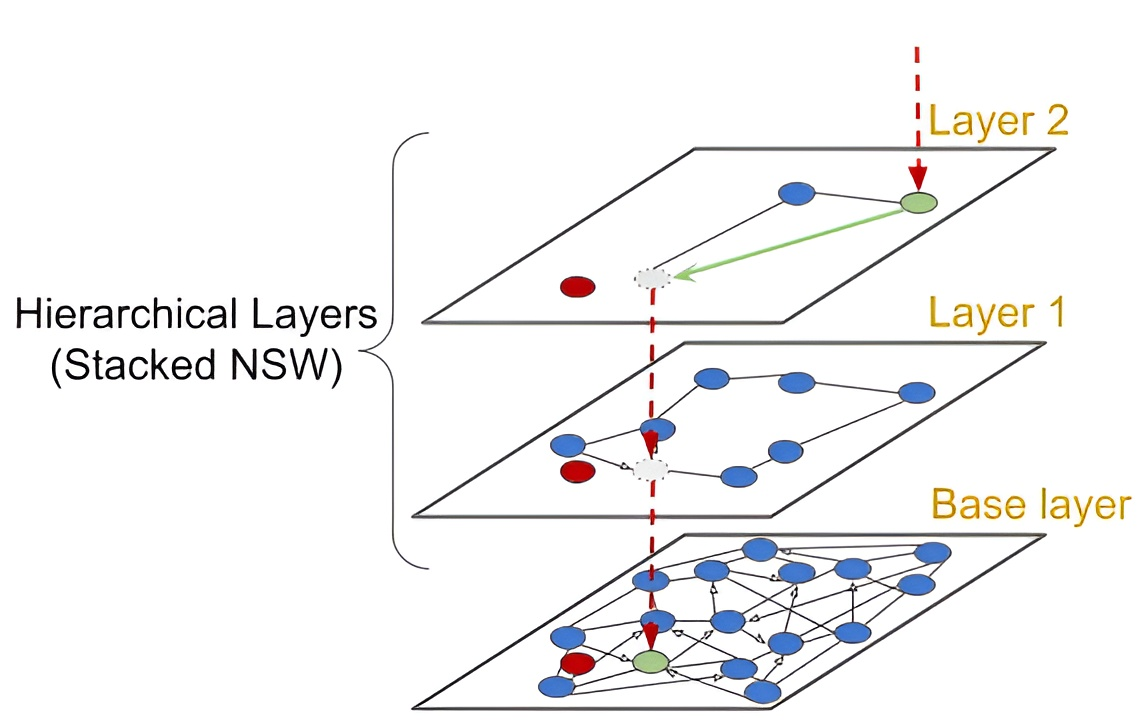
\includegraphics[width=0.7\columnwidth]{../img/graphfamily/snsw.png}
		\caption{Routing through SNSW during search on HNSW graph}        
		\label{fig:snwd}
 \end{figure}




The Stacked-NSW graph is constructed by assigning each node a maximum level L, which is generated using the formula:

\begin{equation} \centering L = \frac{-\ln(\xi)}{\ln\left(M/2\right)} \label{eq:1} \end{equation}

Where $\xi$ is a uniformly random number between 0 and 1, and MM is the maximum outdegree, which controls the probability distribution of a node's maximum layer. The logarithmic nature of the formula ensures that most nodes are concentrated in the lower layers, while only a few nodes reach the top layers.

As M increases, graph connectivity improves, concentrating nodes in the lower layers and reducing the number of hierarchical levels, which minimizes the number of distance calculations required for the beam search. Conversely, smaller values of MM shift more nodes to higher layers, enhancing seed quality for searches on sparse graphs. Table~\ref{tab:layer_distribution} illustrates the distribution of nodes across hierarchical layers for different MM values on the Deep1M dataset.

\begin{table}[ht]
\centering
\caption{Distribution of Nodes Across Hierarchical Layers Based on Outdegree \(M\)}
\label{tab:layer_distribution}
\resizebox{\textwidth}{!}{%
\begin{tabular}{|c|c|c|c|c|c|c|c|c|c|c|}
\hline
\textbf{M} & \textbf{Number of Layers} & \textbf{Layer 1} & \textbf{Layer 2} & \textbf{Layer 3} & \textbf{Layer 4} & \textbf{Layer 5} & \textbf{Layer 6} & \textbf{Layer 7} & \textbf{Layer 8} & \textbf{Layer 9} \\ \hline
5  & 9  & 200058 & 40583 & 7988  & 1581 & 304  & 76   & 11  & 3   & 1   \\ \hline
10 & 6  & 100636 & 10060 & 988   & 116  & 9    & 1    & 0   & 0   & 0   \\ \hline
15 & 5  & 67031  & 4438  & 292   & 18   & 1    & 0    & 0   & 0   & 0   \\ \hline
20 & 4  & 50487  & 2501  & 140   & 7    & 0    & 0    & 0   & 0   & 0   \\ \hline
\end{tabular}%
}
\end{table}

The hierarchical structure enables efficient search by constructing coarse neighborhoods at higher layers, allowing for long jumps in the search space. As the search progresses through lower layers, finer neighborhoods are formed, ultimately leading to the base layer, where the search continues within the most refined region. The search process begins at the highest layer and iteratively moves down through the layers, restarting the search at the next level upon reaching a local minimum, until the optimal entry point for beam search is found at layer 1.

\noindent (2) \textbf{K-D Trees (KD)}: Employed by EFANNA~\cite{efanna}, SPTAG-KDT~\cite{SPTAG2}, and HCNNG~\cite{hcnng}, this approach constructs one or multiple K-D Trees~\cite{kdtree} over a sample of the dataset. During query search, a depth-first search (DFS) traversal is conducted on the K-D Tree(s), providing a set of seed points to initialize the candidate list. The node closest to the query is selected as the entry point for further exploration.

\noindent (3) \textbf{Locality-Sensitive Hashing (LSH)}: Adopted by IEH~\cite{ieh}, LSH constructs a hash-based index on a sample of the dataset. During the search process, this index is used to generate a set of seed points, from which one is chosen as the entry node for the approximate nearest neighbor search.

\noindent (4) \textbf{Medoid (MD)}: Utilized by methods such as DPG~\cite{dpg}, NSG~\cite{nsg}, and Vamana~\cite{vamana}, this approach fixes the medoid node as the entry point during query search. The neighbors of the medoid are used as initial seeds, allowing for efficient exploration of the search space.

\noindent (5) \textbf{Single Fixed Random Entry Point (SF)}: In this strategy, a single random node is pre-selected and fixed as the entry point for all queries. The selected node and its neighbors are used as seed points for search, regardless of the query.

\noindent (6) \textbf{K-Sampled Random Seeds (KS)}: In each query, \(k\) random nodes are selected as seed points to initialize the search. This strategy is implemented in DPG~\cite{dpg}, NSG~\cite{nsg}, and Vamana~\cite{vamana}, where the medoid is combined with randomly chosen nodes to enhance the initial seed set.

\noindent (7) \textbf{Balanced K-means Trees (KM)}: Used by SPTAG-BKT~\cite{SPTAG2}, this method constructs Balanced K-means Trees (BKT)~\cite{bkmtree} over a sample of the dataset. During query search, a depth-first search (DFS) is performed on the BKT structure to retrieve seed points that warm up the candidate list.

In Section~\ref{sec:experiments_ND_SS}, We will compare most common approach for SS in literature, SN, KS, KD, on different datasets and sizes.




\subsection{Neighborhood Diversification}
\label{sec:nd}
In the initial stages of developing graph-based methods for similarity search, techniques such as KGraph proposed approximating the K-nearest neighbor (KNN) graph using NNDescent. This approach relies on iteratively propagating and updating neighborhood lists between connected vertices. Alternatively, NSW presented a graph construction method where nodes are incrementally inserted into the graph. During this process, each node’s neighborhood is retrieved via beam search, and bidirectional edges are established to connect the newly inserted node with those already in the graph. NSW particularly emphasized the importance of long-range edges to ensure efficient search. However, despite some differences in approach, both methods shared a common challenge: achieving good accuracy often required a large outdegree, leading to an increased number of distance calculations during the search.

Since then, several Neighborhood Diversification (ND) techniques have been developed to enhance graph-based data structures for similarity search. We classify graph-based approximate vector search methods that implement various ND strategies into a distinct ND-based class. The primary goal of ND is to create sparse graph structures by pruning unnecessary edges, while maintaining a well-connected network that ensures proximity between nodes. For a given node \( X_q \) and its list of candidate neighbors \( C_q \), the ND step strategically selects specific candidates \( X_i \) for inclusion in \( X_q \)’s neighborhood set \( R_q \). The core principle of ND is to diversify the selection of neighbors, improving the graph's efficiency during search traversal, while preserving the essential proximity relations within the structure.

The need for ND arises because searching a graph where nodes are only connected to their nearest neighbors may involve numerous redundant comparisons before reaching the optimal regions. The concept of ND was initially introduced with the Relative Neighborhood Graph (RNG)~\citep{rng,toussaint02}, which constructs an undirected graph either from scratch or by pruning an existing Delaunay Graph~\cite{dobkin1990delaunay}. In RNG, the longest edge in each triangle formed by three connected points is removed, which reduces redundant connections.

This idea, along with other geometrically motivated strategies, has since been adapted for directed graphs in several modern graph-based approximate similarity search methods~\citep{hnsw,dpg,nsg,nssg,vamana,SPTAG4,elpis}. We have identified three key ND strategies used in these methods: Relative Neighborhood Diversification (RND), Relaxed Relative Neighborhood Diversification (RRND), and Maximum-Oriented Neighborhood Diversification (MOND). 

It is worth noting that ND strategies differ from the small-world network model proposed by Kleinberg~\cite{kleinberg2000, kleinberg2002}, where long-range links are randomly chosen. In contrast, ND implicitly generates long-range links by pruning close neighbors, thus facilitating better traversal of the graph.

Below, we present formal definitions of each method, alongside relevant mathematical expressions and explanations of their operations. Figures~\ref{fig:ND:RND},~\ref{fig:ND:RRND}, and~\ref{fig:ND:MOND} illustrate how each method operates on a candidate neighborhood list.


\subsubsection{Relative Neighborhood Diversification (RND)}
RND was first introduced in the HNSW algorithm~\cite{hnsw} and has been used in other methods like NSG~\cite{nsg}, SPTAG~\cite{SPTAG4}, and ELPIS~\cite{elpis}. This method ensures that a candidate neighbor is added to the neighborhood of the query node only if it is closer to the query than to any already selected neighbors.

\begin{itemize}
    \item \(X_q\) is the query node, i.e., the node to be inserted into the graph.
    \item \(R_q\), the list of current closest neighbors to \(X_q\).
    \item \(C_q\), the list of candidate neighbors to \(X_q\) not yet in \(R_q\).
    \item \(X_j\) is a candidate neighbor being considered for inclusion in \(R_q\) and is part of \(C_q\).
    \item \(X_i\) is a node already in the set \(R_q\).
    \item \(\text{dist}(X_i, X_j)\) represents the Euclidean distance between nodes \(X_i\) and \(X_j\) in the \(d\)-dimensional space.
\end{itemize}

\begin{definition}
\label{def:rnd}
Given a query node \(X_q\), a candidate neighbor \(X_j\) is added to the list \(R_q\) if and only if:
\begin{equation}
    \forall X_i \in R_q, \, \text{dist}(X_q, X_j) < \text{dist}(X_i, X_j)
\end{equation}
\end{definition}

This ensures that redundant edges to nodes closer to each other than to the query node are pruned.

\begin{figure}[h]
    \centering
    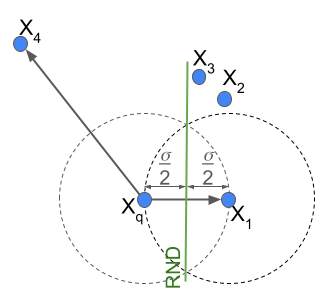
\includegraphics[width=0.4\textwidth]{../img/related/rnd.png}
    \caption{Example of RND pruning applied to the neighborhood list \(C_q\)}
    \label{fig:ND:RND}
\end{figure}

\subsubsection{Relaxed Relative Neighborhood Diversification (RRND)}
RRND, proposed by the Vamana algorithm~\cite{vamana}, relaxes the strict condition of RND by introducing a relaxation factor \(\alpha\). This factor allows nodes to be added to the neighborhood even if they do not strictly satisfy the RND condition, leading to a less aggressive pruning strategy and more neighbors retained.

\begin{itemize}
    \item \(X_q\) is the query node.
    \item \(R_q\), the list of current closest neighbors to \(X_q\).
    \item \(C_q\), the list of candidate neighbors to \(X_q\) not yet in \(R_q\).
    \item \(X_j\) is a candidate neighbor being considered for inclusion in \(R_q\) and is part of \(C_q\).
    \item \(X_i\) is a node already in the set \(R_q\).
    \item \(\alpha\) is the relaxation factor, where \(\alpha \geq 1\).
    \item \(\text{dist}(X_i, X_j)\) represents the Euclidean distance between nodes \(X_i\) and \(X_j\).
\end{itemize}

\begin{definition}
\label{def:rrnd}
Given a relaxation factor \(\alpha\), a candidate neighbor \(X_j\) is added to the list \(R_q\) if:
\begin{equation}
    \forall X_i \in R_q, \, \text{dist}(X_q, X_j) < \alpha \cdot \text{dist}(X_i, X_j)
\end{equation}
\end{definition}

When \(\alpha = 1\), RRND is reduced to RND. This relaxation increases graph connectivity by pruning fewer neighbors.

\begin{figure}[h]
    \centering
    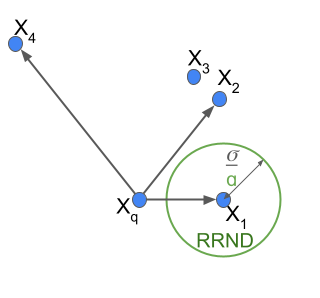
\includegraphics[width=0.4\textwidth]{../img/related/rrnd.png}
    \caption{Example of RRND pruning with relaxation factor \(\alpha = 1.5\)}
    \label{fig:ND:RRND}
\end{figure}

\subsubsection{Maximum-Oriented Neighborhood Diversification (MOND)}
MOND, introduced by DPG~\cite{dpg}, prunes candidate neighbors by focusing on the geometric orientation of edges, ensuring that neighbors are selected to maximize angular separation. This approach prevents the formation of cliques by ensuring that connections span diverse directions in the vector space.

\begin{itemize}
    \item \(X_q\) is the query node.
    \item \(R_q\), the list of current closest neighbors to \(X_q\).
    \item \(C_q\), the list of candidate neighbors to \(X_q\) not yet in \(R_q\).
    \item \(X_j\) is a candidate neighbor being considered for inclusion in \(R_q\) and is part of \(C_q\).
    \item \(X_i\) is a node already in the set \(R_q\).
    \item \(\theta\) is the angle threshold used to guide the pruning process.
    \item \(\angle X_j X_q X_i\) is the angle between the edges \(X_qX_j\) and \(X_qX_i\).
\end{itemize}

\begin{definition}
\label{def:mond}
Given an angle threshold \(\theta\), a candidate neighbor \(X_j\) is added to the list \(R_q\) if:
\begin{equation}
    \forall X_i \in R_q, \, \cos(\angle X_j X_q X_i) < \cos(\theta)
\end{equation}
\end{definition}

This strategy maximizes the angular separation of neighbors in the graph, leading to improved diversity in the neighborhood list.

\begin{figure}[h]
    \centering
    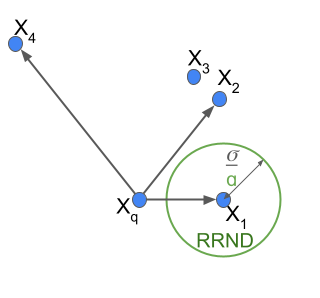
\includegraphics[width=0.4\textwidth]{../img/related/rrnd.png}
    \caption{Example of MOND pruning with angle threshold \(\theta = 60^\circ\)}
    \label{fig:ND:MOND}
\end{figure}

\subsection{Comparison of ND Methods}
As illustrated in Figures~\ref{fig:ND:RND},~\ref{fig:ND:RRND}, and~\ref{fig:ND:MOND}, these three methods vary in how they prune the candidate neighborhood set. RND applies the most stringent pruning criterion, whereas RRND loosens this condition using the relaxation factor \(\alpha\). On the other hand, MOND focuses on maximizing angular separation between neighbors to achieve diversification. These approaches have been demonstrated to enhance both the accuracy and efficiency of graph-based similarity search, with RND and MOND generally offering the optimal balance between computational cost and search accuracy~\cite{gass}.

Below, we prove that both MOND (Maximum-Oriented Neighborhood Diversification) and RRND (Relaxed Relative Neighborhood Diversification) are approximations of RND (Relative Neighborhood Diversification). Furthermore, we show that the converse does not hold, meaning RND does not necessarily approximate MOND or RRND.

\subsubsection{Preliminaries}

We define the necessary variables used in the proof as follows:

\begin{itemize}
    \item \(\mathbf{X}_q\) is the query node, i.e., the node to be inserted into the graph.
    \item \(\mathbf{R}_q\), the list of current closest neighbors to \(\mathbf{X}_q\).
    \item \(\mathbf{C}_q\), the list of candidate neighbors to \(\mathbf{X}_q\) not yet in \(\mathbf{R}_q\).
    \item \(\mathbf{X}_j\) is a candidate neighbor being considered for inclusion in \(\mathbf{R}_q\) and is part of \(\mathbf{C}_q\).
    \item \(\mathbf{X}_i\) is a node already in the set \(\mathbf{R}_q\).
    \item \(\text{dist}(\mathbf{X}_i, \mathbf{X}_j)\) represents the Euclidean distance between nodes \(\mathbf{X}_i\) and \(\mathbf{X}_j\) in the \(d\)-dimensional space.
\end{itemize}

\subsubsection{RRND as an Approximation of RND}

RRND introduces a relaxation factor \(\alpha \geq 1\) that allows edges to be retained even if they would be pruned under RND. The condition for RRND is:

\[
\forall \mathbf{X}_i \in \mathbf{R}_q, \; \text{dist}(\mathbf{X}_q, \mathbf{X}_j) < \alpha \cdot \text{dist}(\mathbf{X}_i, \mathbf{X}_j)
\]

Since \(\alpha \geq 1\), RRND retains more edges than RND. Specifically, if an edge is pruned by RRND, it will also be pruned by RND, but not necessarily the other way around, as RRND allows for more flexible edge retention. This establishes that RRND is an approximation of RND.

\subsubsection{MOND as an Approximation of RND}

MOND prunes edges based on angular separation. It retains neighbors that maximize the angular diversity in the graph. To show that MOND is an approximation of RND, we consider the following nodes:

\begin{itemize}
    \item \(\mathbf{X}_q\) is the query vector.
    \item \(\mathbf{X}_i\) is a neighbor already in \(\mathbf{R}_q\).
    \item \(\mathbf{X}_j\) is a candidate neighbor being considered for inclusion in \(\mathbf{R}_q\).
\end{itemize}

The condition for RND is:

\[
\forall \mathbf{X}_i \in \mathbf{R}_q, \; \text{dist}(\mathbf{X}_q, \mathbf{X}_j) < \text{dist}(\mathbf{X}_i, \mathbf{X}_j)
\]

MOND, however, adds \(\mathbf{X}_j\) to \(\mathbf{R}_q\) if the cosine of the angle between the edges \(\mathbf{X}_q \mathbf{X}_i\) and \(\mathbf{X}_q \mathbf{X}_j\) is less than a threshold \(\cos(\theta)\):

\[
\forall \mathbf{X}_i \in \mathbf{R}_q, \; \cos(\angle \mathbf{X}_i \mathbf{X}_q \mathbf{X}_j) < \cos(\theta)
\]

Where \(\theta\) is the angle threshold (e.g., \( \theta = 60^\circ \)).

\subsection{Proof that MOND Approximates RND}

In this section, we prove that MOND (Maximum-Oriented Neighborhood Diversification) is an approximation of RND (Relative Neighborhood Diversification). MOND aims to maximize the angular separation between edges in the neighborhood list, while RND prunes based on Euclidean distances. We show how the RND condition can be transformed into the angular condition used in MOND.

\subsubsection{Preliminaries}

We define the variables used in the proof:

\begin{itemize}
    \item \(\mathbf{X}_q\) is the query node, i.e., the node to be inserted into the graph.
    \item \(\mathbf{R}_q\) is the list of current closest neighbors to \(\mathbf{X}_q\).
    \item \(\mathbf{C}_q\) is the list of candidate neighbors to \(\mathbf{X}_q\) not yet in \(\mathbf{R}_q\).
    \item \(\mathbf{X}_j\) is a candidate neighbor being considered for inclusion in \(\mathbf{R}_q\).
    \item \(\mathbf{X}_i\) is a node already in the set \(\mathbf{R}_q\).
    \item \(\text{dist}(\mathbf{X}_i, \mathbf{X}_j)\) represents the Euclidean distance between nodes \(\mathbf{X}_i\) and \(\mathbf{X}_j\) in the \(d\)-dimensional space.
\end{itemize}

\subsubsection{RND Condition}

The RND condition states that a candidate neighbor \(\mathbf{X}_j\) is added to the neighborhood \(\mathbf{R}_q\) of \(\mathbf{X}_q\) if:

\[
\text{dist}(\mathbf{X}_q, \mathbf{X}_j) < \text{dist}(\mathbf{X}_i, \mathbf{X}_j), \quad \forall \mathbf{X}_i \in \mathbf{R}_q
\]

This condition ensures that \(\mathbf{X}_j\) is closer to the query node \(\mathbf{X}_q\) than to any existing neighbor \(\mathbf{X}_i\) in \(\mathbf{R}_q\).

\subsubsection{Transition to Angular Condition in MOND}

MOND, on the other hand, uses angular separation between neighbors to decide whether to add \(\mathbf{X}_j\) to \(\mathbf{R}_q\). Specifically, MOND retains \(\mathbf{X}_j\) if the cosine of the angle between the edges \(\mathbf{X}_q \mathbf{X}_i\) and \(\mathbf{X}_q \mathbf{X}_j\) is smaller than a threshold \(\cos(\theta)\), where \(\theta\) is the minimum required angular separation:

\[
\cos(\angle \mathbf{X}_i \mathbf{X}_q \mathbf{X}_j) < \cos(\theta)
\]

To prove that MOND approximates RND, we express the RND condition in terms of angles. Using the cosine law, the distance between two points can be related to the angle between the vectors. The cosine of the angle \(\angle \mathbf{X}_i \mathbf{X}_q \mathbf{X}_j\) can be written as:

\[
\cos(\angle \mathbf{X}_i \mathbf{X}_q \mathbf{X}_j) = \frac{\overrightarrow{\mathbf{X}_q \mathbf{X}_i} \cdot \overrightarrow{\mathbf{X}_q \mathbf{X}_j}}{|\overrightarrow{\mathbf{X}_q \mathbf{X}_i}| \cdot |\overrightarrow{\mathbf{X}_q \mathbf{X}_j}|}
\]

Now, using the Euclidean distances \(\text{dist}(\mathbf{X}_q, \mathbf{X}_i)\) and \(\text{dist}(\mathbf{X}_q, \mathbf{X}_j)\), the dot product of the vectors can be related to these distances. The RND condition implies:

\[
\text{dist}(\mathbf{X}_q, \mathbf{X}_j) < \text{dist}(\mathbf{X}_i, \mathbf{X}_j)
\]

This translates to:

\[
|\overrightarrow{\mathbf{X}_q \mathbf{X}_j}| < |\overrightarrow{\mathbf{X}_i \mathbf{X}_j}|
\]

Therefore, if the distance between \(\mathbf{X}_q\) and \(\mathbf{X}_j\) is small enough, the angle \(\angle \mathbf{X}_i \mathbf{X}_q \mathbf{X}_j\) will be large, ensuring that MOND will retain \(\mathbf{X}_j\) under the angular condition:

\[
\cos(\angle \mathbf{X}_i \mathbf{X}_q \mathbf{X}_j) < \cos(\theta)
\]

Thus, if \(\mathbf{X}_j\) is added by RND, it will also satisfy the angular condition of MOND, proving that MOND is an approximation of RND.

\subsubsection{Counter-Example: RND Does Not Approximate MOND}

To demonstrate that RND does not necessarily approximate MOND, we consider a simple 2D example where:

\[
\mathbf{X}_q = (0, 0), \quad \mathbf{X}_i = (2, 0), \quad \mathbf{X}_j = (1.8, 2.5)
\]

First, calculate the distances:

\[
\text{dist}(\mathbf{X}_q, \mathbf{X}_i) = \sqrt{(2 - 0)^2 + (0 - 0)^2} = 2
\]

\[
\text{dist}(\mathbf{X}_q, \mathbf{X}_j) = \sqrt{(1.8 - 0)^2 + (2.5 - 0)^2} = \sqrt{3.24 + 6.25} \approx 3.08
\]

Since \(\text{dist}(\mathbf{X}_q, \mathbf{X}_j) > \text{dist}(\mathbf{X}_q, \mathbf{X}_i)\), RND would prune \(\mathbf{X}_j\). Now, calculate the angle for MOND:

\[
\overrightarrow{\mathbf{X}_q \mathbf{X}_i} = (2, 0), \quad \overrightarrow{\mathbf{X}_q \mathbf{X}_j} = (1.8, 2.5)
\]

\[
\overrightarrow{\mathbf{X}_q \mathbf{X}_i} \cdot \overrightarrow{\mathbf{X}_q \mathbf{X}_j} = 2 \cdot 1.8 + 0 \cdot 2.5 = 3.6
\]

\[
|\overrightarrow{\mathbf{X}_q \mathbf{X}_i}| = 2, \quad |\overrightarrow{\mathbf{X}_q \mathbf{X}_j}| \approx 3.08
\]

\[
\cos(\theta) = \frac{3.6}{2 \times 3.08} \approx 0.586
\]

Since \( \cos(60^\circ) = 0.5 \), MOND will retain \(\mathbf{X}_j\), but RND would have pruned it. Therefore, MOND approximates RND, but RND does not always approximate MOND.



\subsubsection{Counter-Example: RND Does Not Approximate MOND}

To demonstrate that RND does not necessarily approximate MOND, consider a case in 2D where:

\[
\mathbf{X}_q = (0, 0), \quad \mathbf{X}_i = (2, 0), \quad \mathbf{X}_j = (1.8, 2.5)
\]

First, calculate the distances:

\[
\text{dist}(\mathbf{X}_q, \mathbf{X}_i) = \sqrt{(2 - 0)^2 + (0 - 0)^2} = 2
\]

\[
\text{dist}(\mathbf{X}_q, \mathbf{X}_j) = \sqrt{(1.8 - 0)^2 + (2.5 - 0)^2} = \sqrt{3.24 + 6.25} \approx 3.08
\]

Since \(\text{dist}(\mathbf{X}_q, \mathbf{X}_j) > \text{dist}(\mathbf{X}_q, \mathbf{X}_i)\), RND will prune \(\mathbf{X}_j\). Now, calculate the angle for MOND:

\[
\overrightarrow{\mathbf{X}_q \mathbf{X}_i} = (2, 0), \quad \overrightarrow{\mathbf{X}_q \mathbf{X}_j} = (1.8, 2.5)
\]

\[
\overrightarrow{\mathbf{X}_q \mathbf{X}_i} \cdot \overrightarrow{\mathbf{X}_q \mathbf{X}_j} = 2 \cdot 1.8 + 0 \cdot 2.5 = 3.6
\]

\[
|\overrightarrow{\mathbf{X}_q \mathbf{X}_i}| = 2, \quad |\overrightarrow{\mathbf{X}_q \mathbf{X}_j}| \approx 3.08
\]

\[
\cos(\theta) = \frac{3.6}{2 \times 3.08} \approx 0.586
\]

Since \( \cos(60^\circ) = 0.5 \), MOND will not prune \(\mathbf{X}_j\), but RND would have pruned it. Hence, MOND is not fully approximated by RND.




 




\section{Taxonomy of State-of-the-Art Graph-Based Approaches for Approximate Vector Search}

Figure~\ref{fig:roadmap} illustrates the classification of state-of-the-art graph-based methods, categorized into five fundamental design paradigms: Seed Selection (SS), Neighborhood Propagation (NP), Incremental Insertion (II), Neighborhood Diversification (ND), and the Divide-and-Conquer (DC) strategy.

\begin{figure}[ht] 
\centering
		\captionsetup{justification=centering}
		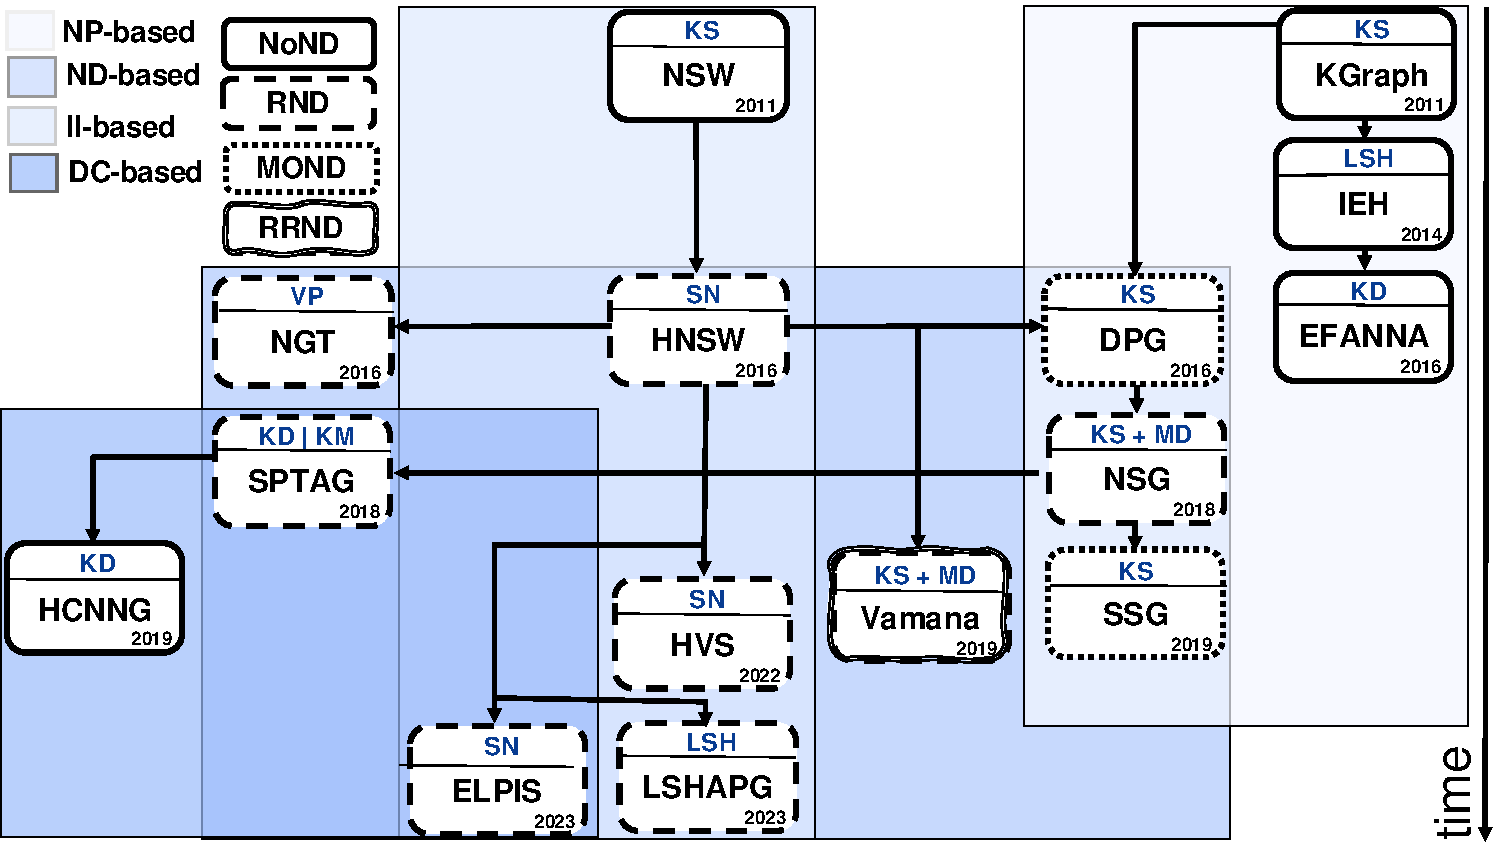
\includegraphics[width=\columnwidth]{../img/graphfamily/RoadMAPGANNS.pdf}
		\caption{Graph-Based Approximate Indexing Paradigms}        
		\label{fig:roadmap}
\end{figure}
The taxonomy further illustrates the evolution of these methods over time, with directed arrows showing how certain approaches have influenced others. Within the ND category, different strategies are highlighted, including No Neighborhood Diversification (NoND), RND, RRND, and MOND. Each method's Seed Selection (SS) strategy is also represented, such as KS, KD, SN, MD, LSH, and KM. (SF is proposed in this work but has not yet been adopted by existing methods.) Some methods incorporate multiple strategies, as seen in NSG and VAMANA, which leverage both KS and MD, or SPTAG, which alternates between KD and KM. Notably, many methods can integrate more than one paradigm. For example, HNSW combines Incremental Insertion (II) with neighborhood pruning using RND, thus falling into both II and ND categories.
KGraph~\cite{kgraph} was the first approach to employ NP for approximating the exact k-NN graph (k-NNG), which has quadratic complexity, and it subsequently influenced several methods like IEH~\cite{ieh} and EFANNA~\cite{efanna}. Concurrently, NSW~\cite{nsw11} introduced the II strategy for graph construction, which was later refined by HNSW~\cite{hnsw} and DPG~\cite{dpg} through the integration of ND to enhance the performance of NSW and KGraph, respectively.

The effectiveness of HNSW and DPG motivated other methods to adopt ND, such as NSG~\cite{nsg} and SSG~\cite{nssg}, which applied ND on the NP-based graph created by EFANNA~\cite{efanna}. SPTAG~\cite{SPTAG4} combined the DC paradigm with ND, while Vamana~\cite{vamana} followed NSG’s lead by constructing the graph via beam search, applying both RRND and RND in two rounds of pruning. HCNNG~\cite{hcnng}, inspired by SPTAG, incorporated a DC approach without employing ND. Similarly, ELPIS~\cite{elpis}, while using DC, leveraged both II and ND.

Earlier methods, with the exception of NSW, predominantly relied on NP. However, more recent efforts have shifted towards leveraging the ND, II, and DC paradigms due to their superior performance~\cite{aumuller2017ann, shimomura2021survey, graph-survey-vldb}, which will be further illustrated in Chapter~\ref{sec:experiments}.

In the next section, we will review the state-of-the-art techniques for in-memory graph-based approximate vector search.

\subsection{State-of-the-Art Approaches} 

\noindent{\bf KGraph}~\cite{kgraph} reduces the construction complexity of an exact k-NNG, which is quadratic in the worst case. It constructs an approximate k-NNG by refining a randomly initialized graph with an empirical time complexity of \( O(n^{1.14}) \)~\cite{nndescent}. This refinement process, referred to as NNDescent~\cite{nndescent} (Neighborhood Propagation), improves the approximation of the \( k \)-NN graph based on the assumption that a vertex's neighbors are more likely to be neighbors of each other. The process iterates over all vertices in the graph, and for each vertex \( u \), it considers every pair \( (x,y) \) of its neighbors. It adds \( x \) to the neighbors of \( y \) and vice versa, retaining only the closest \( k \) neighbors for each vertex.

\noindent{\bf Iterative Expanding Hashing (IEH)}~\cite{ieh} follows a similar process to KGraph in building an approximate k-NNG but generates initial candidates for each node using a hashing function. Two extensions of IEH, IEH-LSH~\cite{iehlsh} and IEH-ITQ~\cite{iehitq}, were proposed to improve the effectiveness of the initial candidates through more advanced hashing techniques. All these methods refine the graph using NNDescent~\cite{nndescent}.

\noindent{\bf EFANNA}~\cite{efanna} adopts seed selection and candidate refinement similar to KGraph~\cite{kgraph} and IEH~\cite{ieh}. It builds an approximate k-NNG by initially selecting the neighbors of each vertex through randomized truncated K-D Trees~\cite{dasgupta2008random}, and then applies NNDescent~\cite{nndescent} to refine the graph. During search, EFANNA utilizes these pre-built trees to retrieve initial seeds and then performs beam search on the graph index.

\noindent{\bf Navigable Small World (NSW)}~\cite{nsw11,nsw14} approximates a Delaunay graph that guarantees the small-world property~\cite{watts98}, where the number of hops \(L\) between two randomly chosen vertices grows logarithmically with the graph size \(n\), i.e., \(L \propto \log(n)\). NSW is derived from the VoroNet graph~\cite{voronet}, an extension of Kleinberg's small-world model~\cite{kleinberg2000,kleinberg2002}. The VoroNet graph is incrementally built by inserting randomly selected vertices and connecting them to \(2d+1\) neighbors chosen through beam search on the existing vertices. The early edges act as long-range connections, facilitating rapid traversal~\cite{voronet}, and the resulting graph ensures small-world properties~\cite{voronet,beaumont07}.

\noindent{\bf Hierarchical Navigable Small World (HNSW)}~\cite{hnsw} addresses the scalability limitations of NSW~\cite{nsw11,nsw14} by proposing the use of RND for neighborhood pruning and a multi-hierarchical seed selection strategy (SN). Each hierarchical layer contains a subgraph of the layer beneath it, with the base layer covering the entire dataset \( \mathbb{S} \). HNSW incrementally builds an NSW graph but refines candidate neighbors in each layer using RND. During query search, HNSW leverages SN to quickly locate an entry point in the base layer, from which beam search is initiated.

\noindent{\bf Diversified Proximity Graph (DPG)}~\cite{dpg} extends KGraph~\cite{kgraph} by introducing a diversification technique known as Maximum-Oriented Neighborhood Diversification (MOND), which maximizes the angles between neighbors to create a sparser graph. MOND is applied iteratively to all nodes, and the directed graph is then converted into an undirected graph for improved connectivity. Despite MOND being the focus, DPG's public implementation~\cite{dpgrepo} actually employs RND for neighborhood diversification instead of MOND.

\noindent{\bf Navigating Spreading-out Graph (NSG)}~\cite{nsg} also builds an approximate k-NNG but constructs an EFANNA graph instead of a KGraph. NSG diversifies its graph using RND and constructs a depth-first search (DFS) tree to ensure the graph's connectivity. Any disconnected vertices are linked to their nearest connected vertex to maintain overall graph structure.

\noindent{\bf Vamana}~\cite{vamana} follows a similar approach to NSG, utilizing visited nodes to build long-range edges. However, Vamana begins by creating a random graph with node degrees \( \geq \log(n) \) to ensure initial graph connectivity~\cite{erconnect}. A beam search is performed for each node, and the visited nodes are refined using RRND. Bi-directional edges are added, and the neighborhood list is further pruned using RND. The process is repeated to enhance graph quality, applying RRND in the second round to increase graph connectivity.

\noindent{\bf SSG}~\cite{nssg} integrates the MOND strategy from DPG~\cite{dpg} and mirrors the construction methods of NSG~\cite{nsg} and DPG~\cite{dpg}. Rather than searching each node for candidates, SSG uses breadth-first search (BFS) to gather candidate neighbors through local expansion on a base graph (EFANNA). When the maximum candidate list size is reached, SSG applies MOND to prune neighbors forming small angles (below a threshold \( \theta \)) with existing neighbors. Multiple DFS trees are built from different random points to enhance connectivity, compared to NSG's single DFS tree.

\noindent{\bf NGT}~\cite{ngt_library} is an approximate nearest neighbor (ANN) search library developed by Yahoo Japan. It offers two construction methods: one extends KNN graphs with reverse edges, forming bi-directed KNN graphs~\cite{ngtpanng1}, while the other incrementally builds graphs similar to HNSW with a range-based search strategy~\cite{ngtpanng2}.  In this study, we consider the former~\cite{ngtpanng1}. Additionally, the library includes methods that employ quantization for highly efficient search.
NGT maintains efficiency by pruning neighbors via RND and using Vantage-Point Trees~\cite{vptree} to select seed nodes for accurate query results

\noindent{\bf SPTAG}~\cite{SPTAG4}, developed by Microsoft, follows a divide-and-conquer (DC) approach. SPTAG selects small dataset samples and builds K-D Trees~\cite{kdtree} or Balanced K-means Trees~\cite{bkmtree}, which are used for seed selection. The full dataset is clustered using TP Trees~\cite{tptree}, and exact k-NN graphs are built and refined using ND for each cluster. The graphs are merged to form a single large graph for query processing.

\noindent{\bf Hierarchical Clustering-based Nearest Neighbor Graph (HCNNG)}~\cite{hcnng}, inspired by SPTAG, uses hierarchical clustering to divide the dataset into overlapping subsets. Each subset forms a Minimum Spanning Tree (MST), and the vertices and edges from all MSTs are merged to construct a unified graph. To aid search, HCNNG builds multiple K-D Trees~\cite{kdtree} to identify initial entry points during query processing.

\noindent{\bf HVS}~\cite{hvs} extends HNSW's base layer by refining the construction of hierarchical layers. Instead of random selection, nodes are assigned to layers based on local density to better capture data distribution. Each layer forms a Voronoi diagram, with nodes representing Voronoi cells, 
and uses multi-level quantization, increasing dimensionality by a factor of 2 in each lower layer.
%\(2^i\) at each lower layer, and i is the number of the layer. 
Search at the base layer is similar to that of HNSW.
%, ensuring accurate nearest neighbor retrieval while maintaining efficiency across layers.

\noindent{\bf LSHAPG}~\cite{lshapg} combines HNSW graphs with multiple hash tables based on the LSB-Tree structure~\cite{lsb} to enhance search efficiency. It leverages $L$ hash tables to retrieve seeds for beam search on the base layer, unlike HNSW, which selects a single seed through SN. LSHAPG also utilizes these hash tables for probabilistic routing during search, pruning neighbors based on the projected distance %between its projection and the query’s projection 
before evaluating and pruning the raw vectors.
%to reduces the computational cost of neighbor pruning during beam search.


\noindent{\bf ELPIS}~\cite{elpis}, our proposed approach for approximate vector search, employs a divide-and-conquer strategy. ELPIS partitions the dataset into multiple subsets using the Hercules EAPCA tree~\cite{hercules}, with each leaf corresponding to a different subset. A graph-based index is then constructed in parallel for each leaf using HNSW~\cite{hnsw}. During search, ELPIS heuristically selects an initial cluster via DFS traversal of the EAPCA tree and initiates beam search on the corresponding graph.

In the following chapter, we provide a detailed explanation of ELPIS and present a comparative analysis of state-of-the-art methods across various datasets and scales. Additionally, the next section will focus on experiments examining different approaches to seed selection and neighborhood diversification, along with a theoretical and empirical analysis of beam search complexity across graph-based methods.

\section{Experimental Evaluation}
\label{sec:experiments_ND_SS}

In this section, we present an evaluation of the various seed selection and neighborhood diversification methods. To isolate the effects of each strategy, we first implement a basic Incremental Insertion (II) method, where nodes are inserted incrementally. Each node \(i\) obtains its list of candidate neighbors through a beam search on the current partial graph containing the previously inserted nodes. Subsequently, we apply each strategy individually to the resulting graph.

We conduct tests using both real-world and synthetic datasets: (i) \emph{Deep}~\cite{url/data/deep1b}, which contains 1 billion vectors of 96 dimensions extracted from the final layers of a convolutional neural network; (ii) \emph{Sift}~\cite{conf/icassp/jegou2011,url/data/sift}, consisting of 1 billion 128-dimensional SIFT vectors representing image features; and (iii) synthetic datasets generated randomly, comprising RandPow0, RandPow5, and RandPow50, each with 256 dimensions, generated according to a power law distribution~\cite{powerlaw} using exponents of 0 (uniform~\cite{url/power-law}), 5, and 50 (highly skewed distributions). Power law distributions, expressed as \(Y = kX^a\), model many real-world phenomena (e.g., in economics, biology, social networks). The skewness of the distribution increases with \(a\), where \(a = 0\) represents a uniform distribution.

We experiment with subsets of various sizes from the real datasets, referring to each by its name and size in gigabytes (e.g., Deep25GB). For the largest datasets, we use the 1M and 1B prefixes to refer to 1-million and 1-billion vector subsets, respectively.

The query sets contain 100 individual vectors, processed one at a time to simulate real-world query scenarios where queries arrive unpredictably~\cite{itsawreport,DBLP:conf/edbt/GogolouTPB19,conf/sigmod/gogolou20}. In cases where results are reported for 1 million queries, these are extrapolated from the 100-query sets. For Deep and Sift, queries are randomly sampled from the available query workloads.

We measure the number of \textit{distance calculations} required to answer each query. Additionally, we assess the accuracy of each \(k\)-NN query using \textit{Recall}, which reflects the proportion of true nearest neighbors that the query \(S_Q\) successfully retrieves.

\subsection{Neighborhood Diversification}
\label{subsec:experiments-ND}

We now assess the performance of the neighborhood diversification (ND) strategies introduced in Section~\ref{sec:nd}, namely RND, RRND, and MOND, compared against a baseline with no neighborhood diversification (NoND). Each strategy is applied independently to an II-based graph, where nodes are inserted sequentially, and each node is connected to a pruned list of neighbors. The list is determined through beam search with a maximum outdegree of \(R = 60\) and a beam width of \(L = 800\). Bi-directional edges are created between neighbors, and the neighborhood list is pruned down to \(R\) neighbors using the corresponding ND strategy.

Graphs are built on the Deep and Sift datasets with sizes of 25GB, 100GB, and 1B. For RRND and MOND, we test various values of \(\alpha\) (ranging from 1 to 2) and \(\theta\) (ranging from \(50^\circ\) to \(80^\circ\)), respectively. The values \(\alpha = 1.3\) and \(\theta = 60^\circ\) are used in the final experiments, as they yield the best results. Each workload consists of 100 queries, and we evaluate the trade-off between accuracy and efficiency by measuring recall and the number of distance calculations performed during search.

\noindent{\textbf{Pruning Ratio.}} In the previous section, we demonstrated that RND applies more aggressive pruning compared to RRND, which relaxes the pruning condition using the parameter \(\alpha\), and MOND, as established through our theoretical proofs. Our theoretical findings align with the empirical pruning ratios of the three methods, as depicted in Figure \ref{fig:pruning_ratio}. The figure illustrates the average pruning ratio across nodes during graph construction for the Deep and Sift 25GB datasets:

\begin{figure}[h]
    \centering
    \captionsetup{justification=centering}
    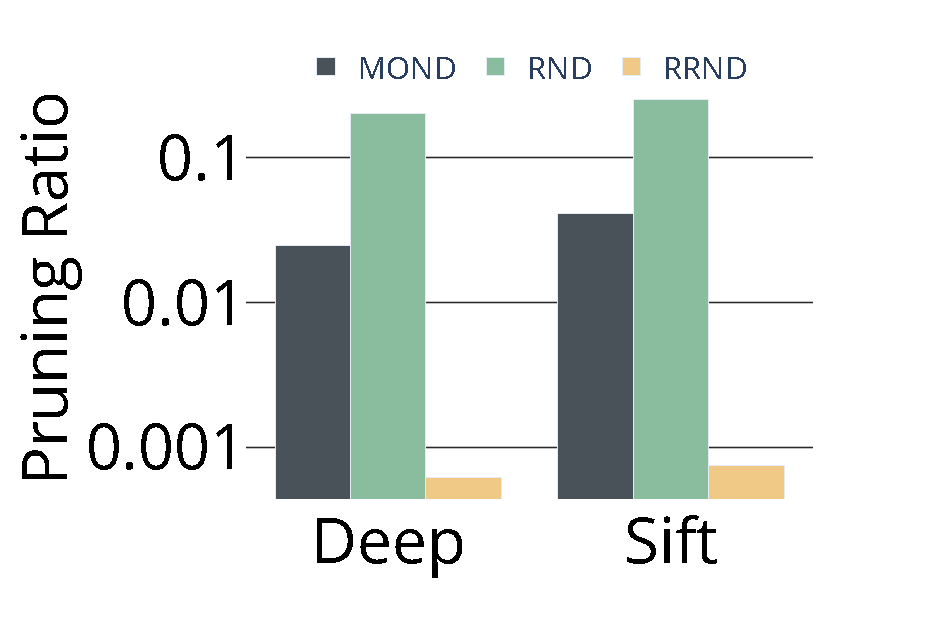
\includegraphics[width=0.5\textwidth]{../img/Experiments/RNG/pruningratio_n.pdf}
    \caption{Average pruning ratio across nodes during graph building for 25GB datasets.}
    \label{fig:pruning_ratio}
\end{figure}

During graph construction using incremental insertion, the pruning ratio is calculated for each node based on the KNN results obtained by performing a beam search on the partial graph of already inserted nodes. This candidate neighbors list is then pruned based on the neighborhood diversification method. The pruning ratio is defined as the ratio of the candidate neighbors list size before and after the pruning process. A lower value indicates less pruning, while a higher value signifies more aggressive pruning.

In both the Deep and Sift datasets, our empirical results show that RND achieves the highest pruning ratio, with 20\% and 25\% respectively. MOND comes second with 2\% and 4\%, while RRND, with a default value of \(\alpha = 1.5\), prunes the least, at 0.6\% and 0.7\%, respectively, in the Deep and Sift datasets.

\noindent{\textbf{Comparison of Query Performance on Real-world Datasets.}}
Figure~\ref{fig:ND:search:real} shows that both RND and MOND consistently outperform RRND, while NoND performs the worst across all datasets. As the dataset size increases, the performance gap between NoND and the ND-based methods widens, especially at high recall levels (Figures \ref{fig:ND:sift1b} and \ref{fig:ND:deep1b}). This is due to the increased number of hops required to find nearest neighbors and the dense neighborhoods formed in the NoND method, where no pruning is applied.

These results emphasize the critical role of the ND paradigm in enhancing query-answering performance, with RND and MOND emerging as the most effective strategies.

\begin{figure}[h!]
	\captionsetup{justification=centering}
	\centering	
		\begin{subfigure}{\columnwidth}
			\centering
			\captionsetup{justification=centering}	
			
\includegraphics[width=0.4\columnwidth]{../img/Experiments/RNG/legend.png}
			\label{fig:ND:legend}
		\end{subfigure}\\
		\begin{subfigure}{0.28\columnwidth}
			\centering
			\captionsetup{justification=centering}	
			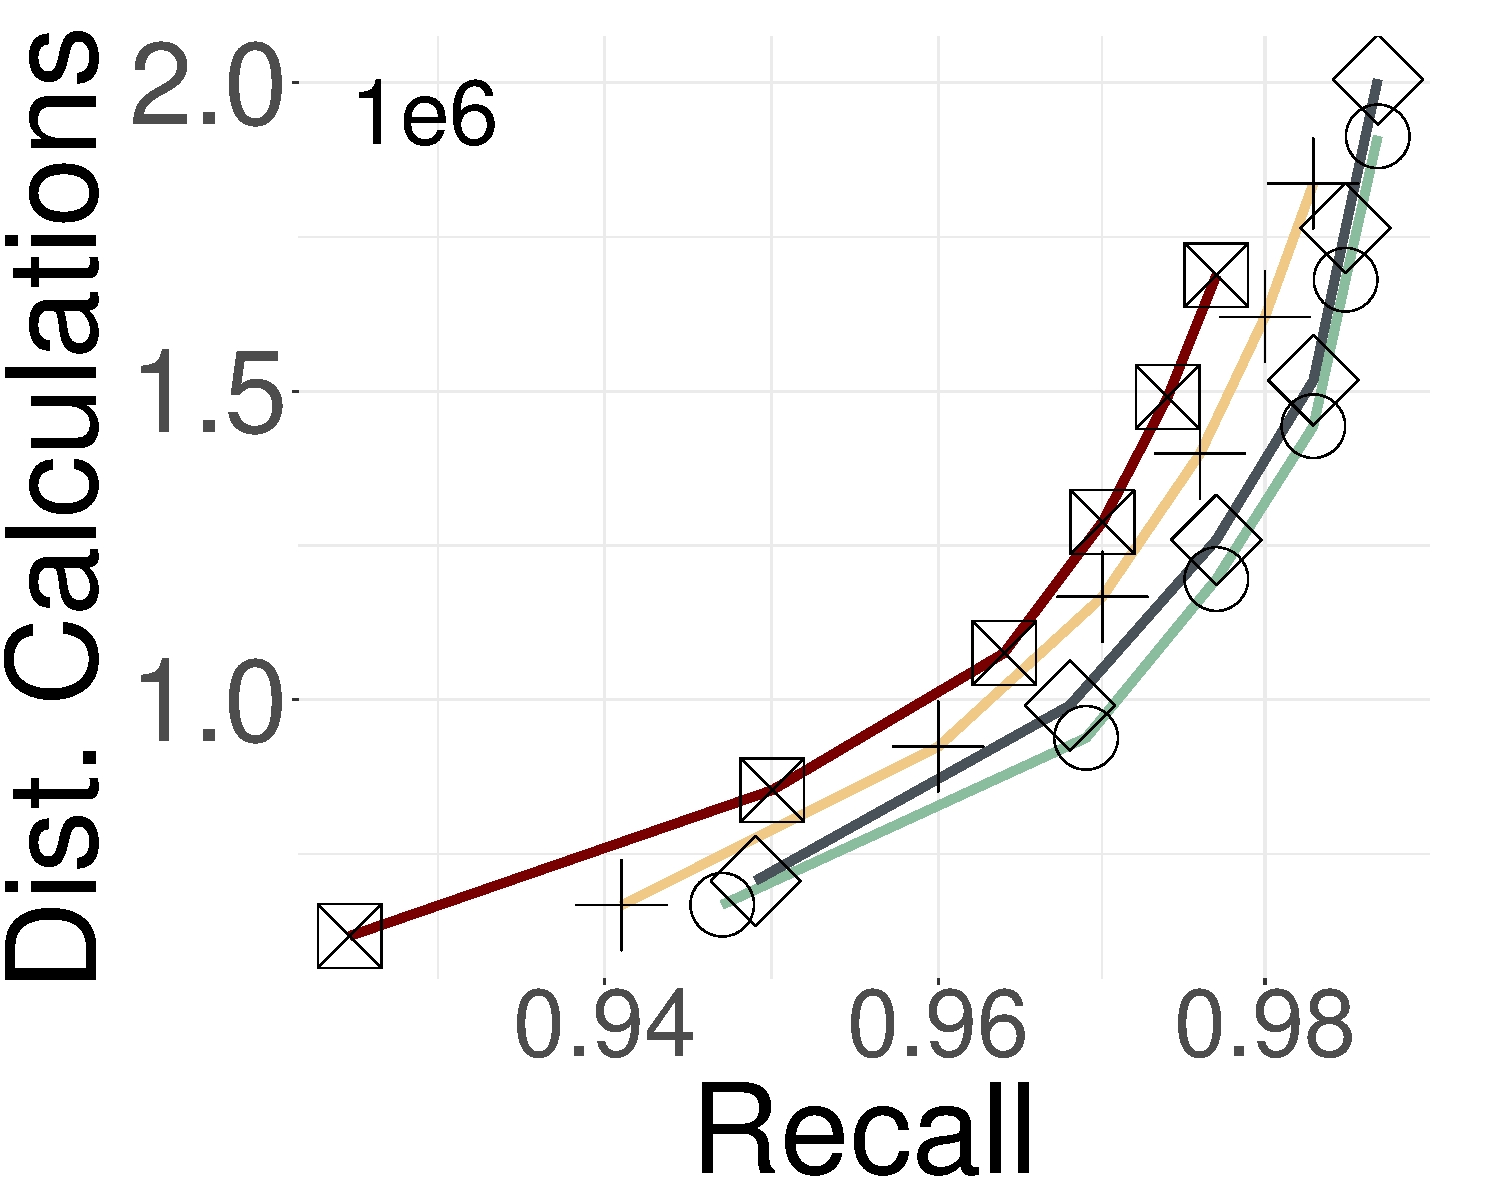
\includegraphics[width=\textwidth]{../img/Experiments/RNG/DC_DEEP25GB.pdf}
		\caption{{DEEP25GB}}
		\label{fig:ND:deep25GB}	
		\end{subfigure}	
  \hspace{0.5cm}
		\begin{subfigure}{0.28\columnwidth}
			\centering
			\captionsetup{justification=centering}	
			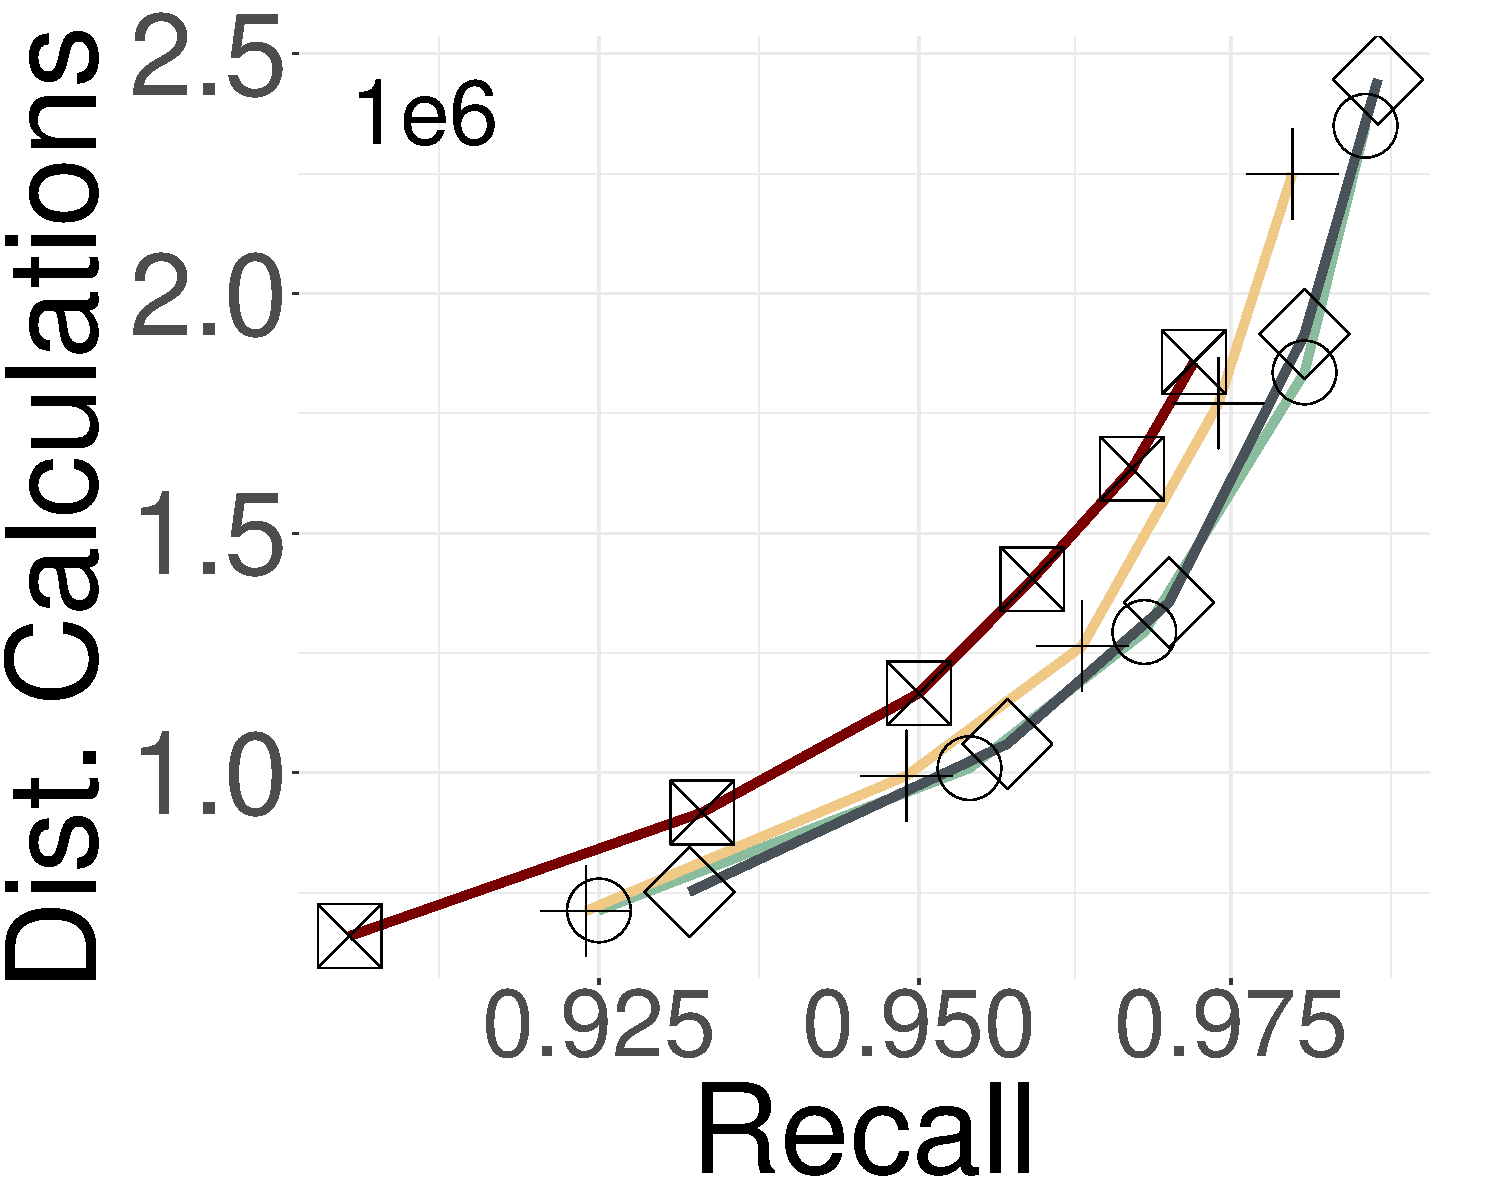
\includegraphics[width=\textwidth]{../img/Experiments/RNG/DC_DEEP100GB.pdf}
		\caption{{DEEP100GB}}
		\label{fig:ND:deep100GB}
		\end{subfigure}	
  \hspace{0.5cm}
		\begin{subfigure}{0.28\columnwidth}
			\centering
			\captionsetup{justification=centering}	
			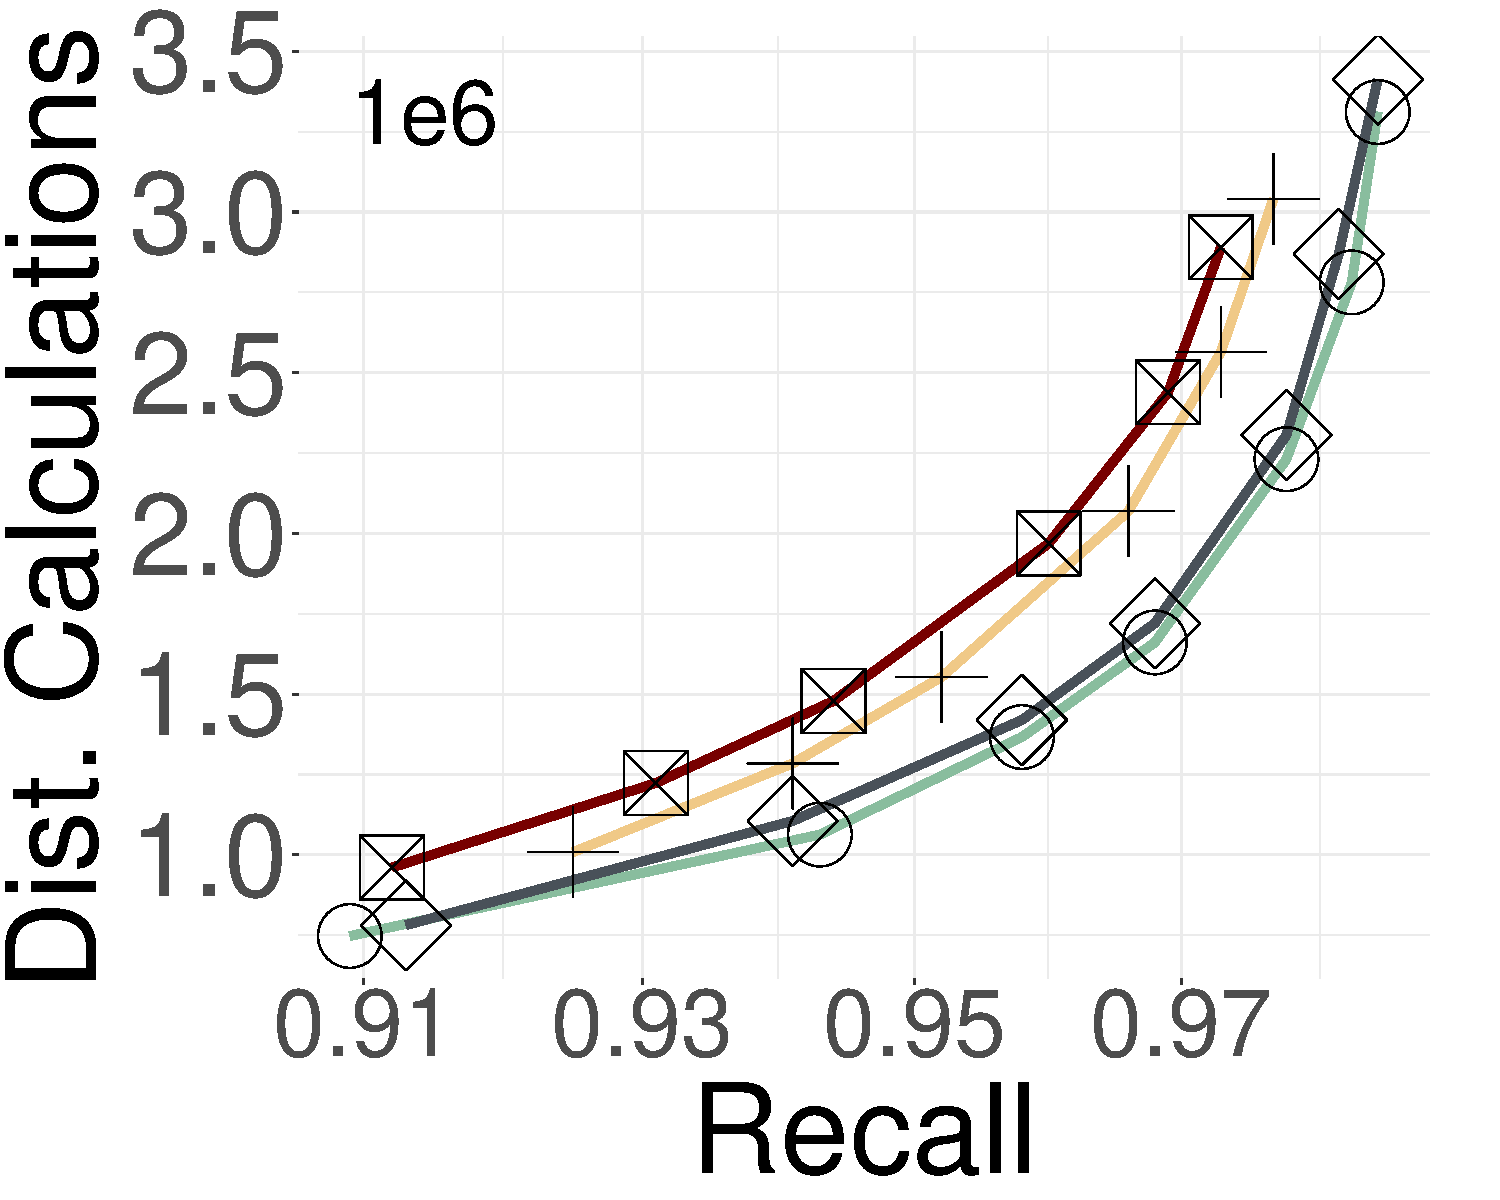
\includegraphics[width=\textwidth]{../img/Experiments/RNG/DC_DEEP1B.pdf}
		\caption{{DEEP1B}}%need to be updated
		\label{fig:ND:deep1b}	
  \end{subfigure}	
 
		\begin{subfigure}{0.28\columnwidth}
			\centering
			\captionsetup{justification=centering}	
			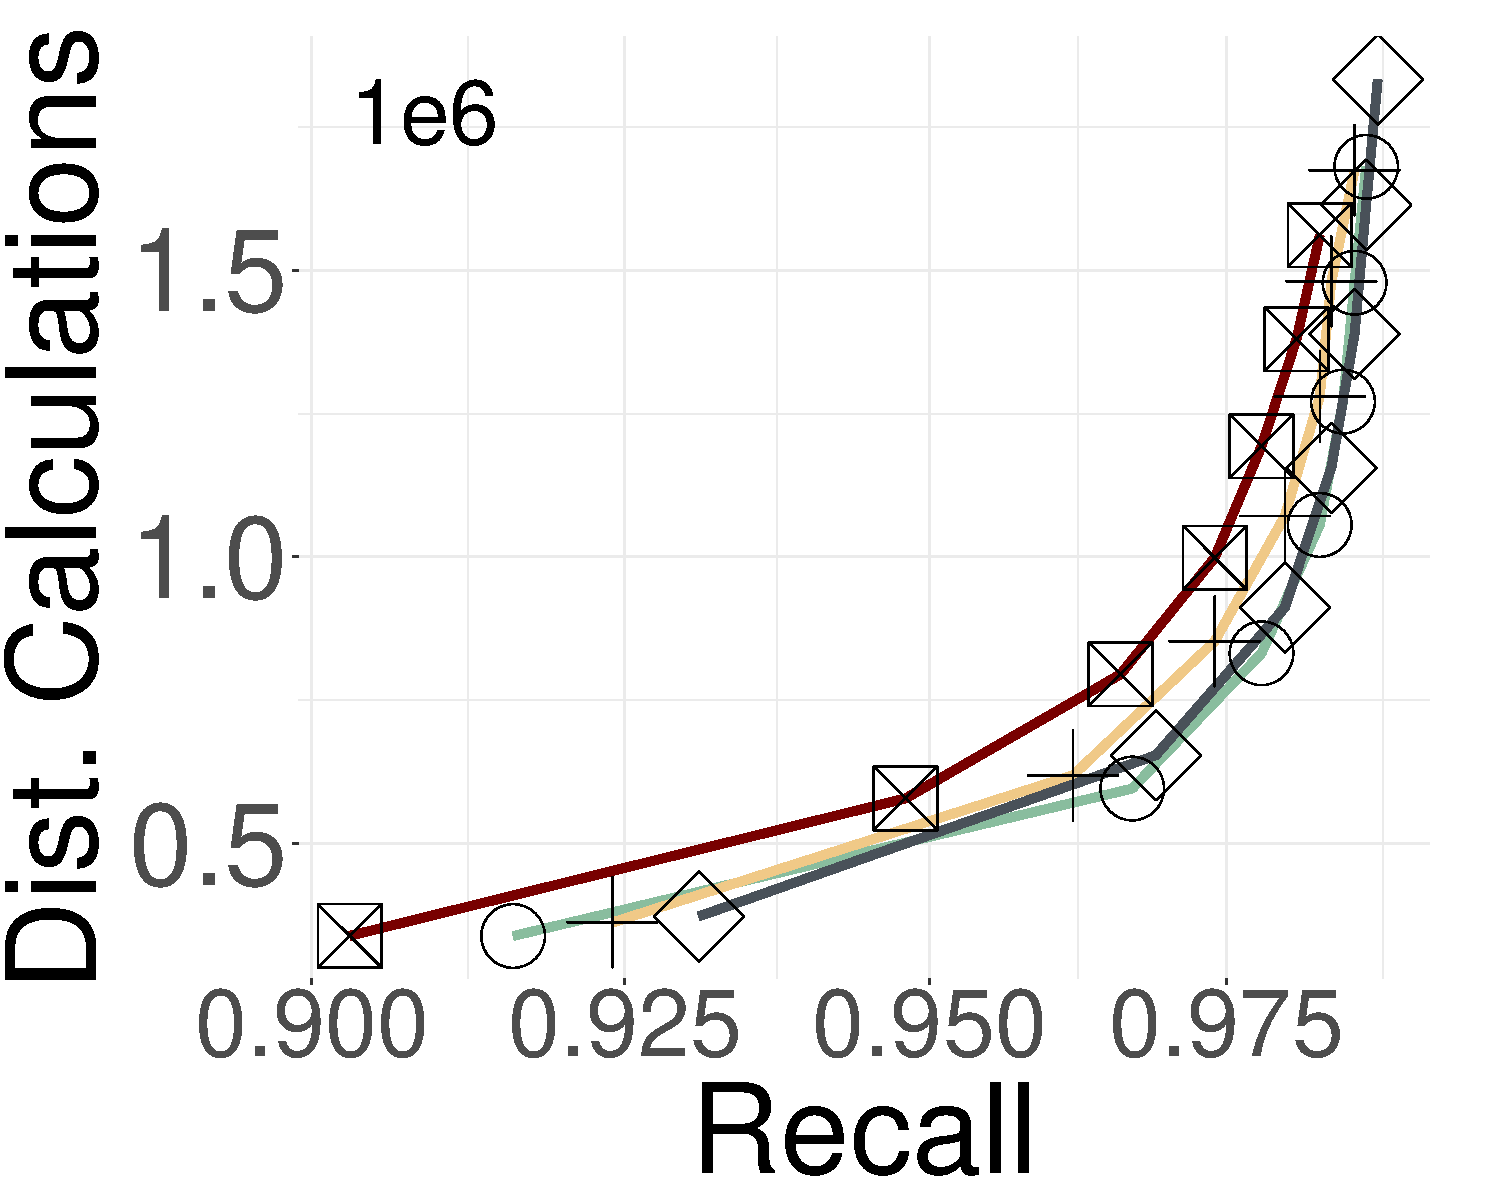
\includegraphics[width=\textwidth]{../img/Experiments/RNG/DC_SIFT25GB.pdf}
   \caption{{SIFT25GB}}
		\label{fig:ND:sift25GB}
		\end{subfigure}	
  \hspace{0.5cm}
		\begin{subfigure}{0.28\columnwidth}
			\centering
			\captionsetup{justification=centering}	
			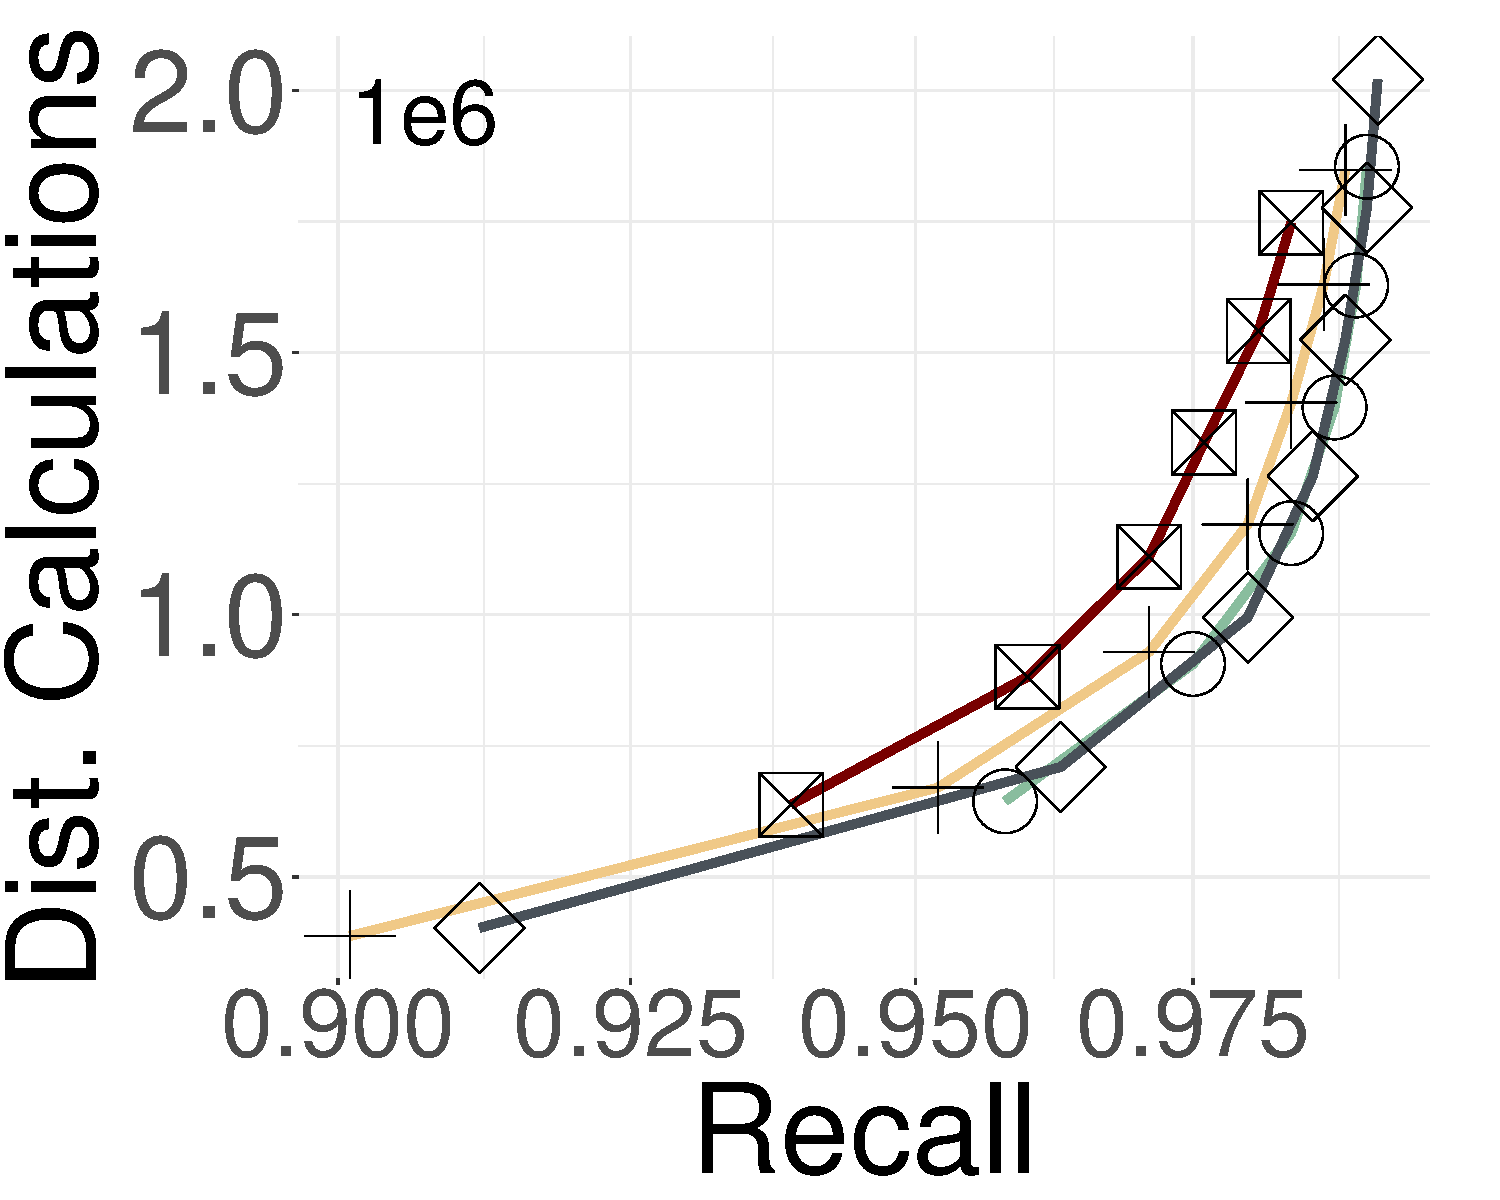
\includegraphics[width=\textwidth]{../img/Experiments/RNG/DC_SIFT100GB.pdf}
             \caption{{SIFT100GB}}
		      \label{fig:ND:sift100GB}
		\end{subfigure}	
  \hspace{0.5cm}
		\begin{subfigure}{0.28\columnwidth}
			\centering
			\captionsetup{justification=centering}	
			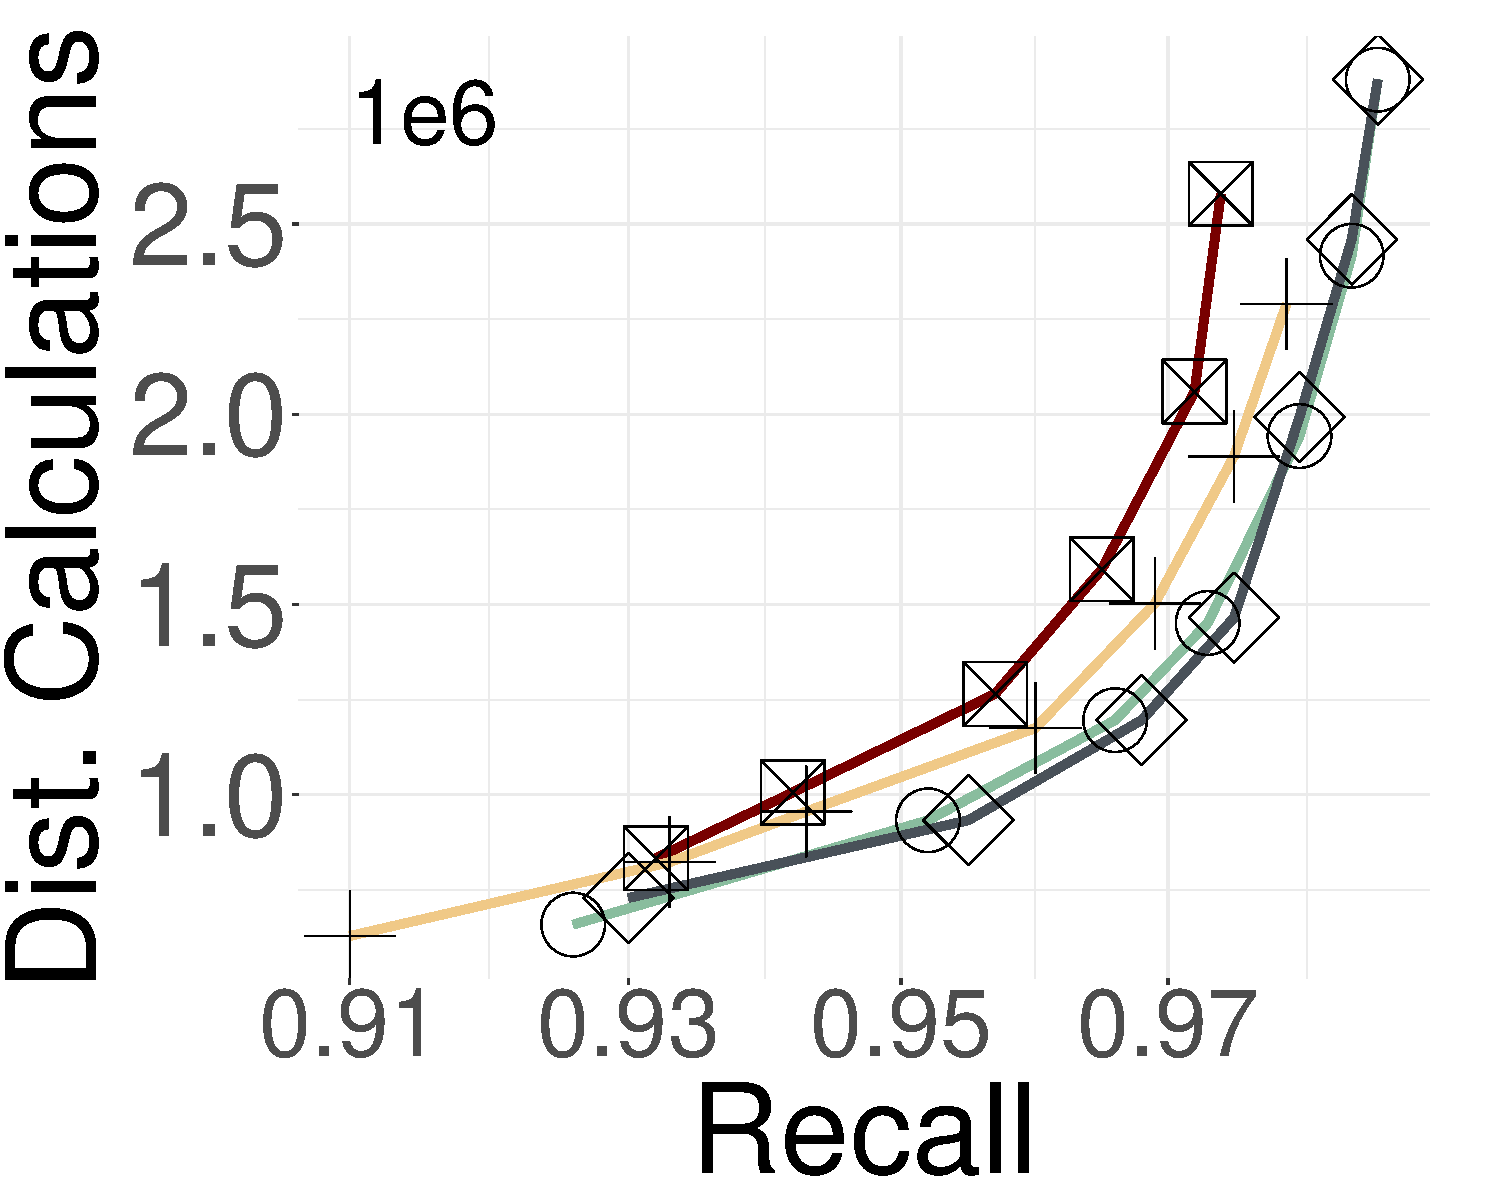
\includegraphics[width=\textwidth]{../img/Experiments/RNG/DC_SIFT1B.pdf}
   \caption{{SIFT1B}}
		\label{fig:ND:sift1b}
		\end{subfigure}	
		\caption{{ND methods performance on real-world datasets}}
		\label{fig:ND:search:real}
 \end{figure}

We compare different ND approaches with II based graph across random dataset with different skewness, Pow1, Pow5 and Pow50 25GB datasets. 

  \noindent{\textbf{Comparison of Query performance on Random Dataset}} Figure~\ref{fig:RNG:search:pow} shows that the three ND strategies have comparable performance when the data distribution is uniform (Pow1), but when the distribution is skewed, MOND takes the lead and RRND becomes competitive with RND. We believe that MOND exhibits a superior performance because on the highly-skewed datasets, the distribution is concentrated within a specific region, thus the orientation pruning of MOND becomes more effective.


\begin{figure}[h!]
	\captionsetup{justification=centering}
	\centering	
		\begin{subfigure}{\columnwidth}
			\centering
			\captionsetup{justification=centering}	
			
\includegraphics[width=0.4\columnwidth]{../img/Experiments/RNG/legend.png}
			\label{fig:RNG:legend}
		\end{subfigure}\\
		\begin{subfigure}{0.28\columnwidth}
			\centering
			\captionsetup{justification=centering}	
			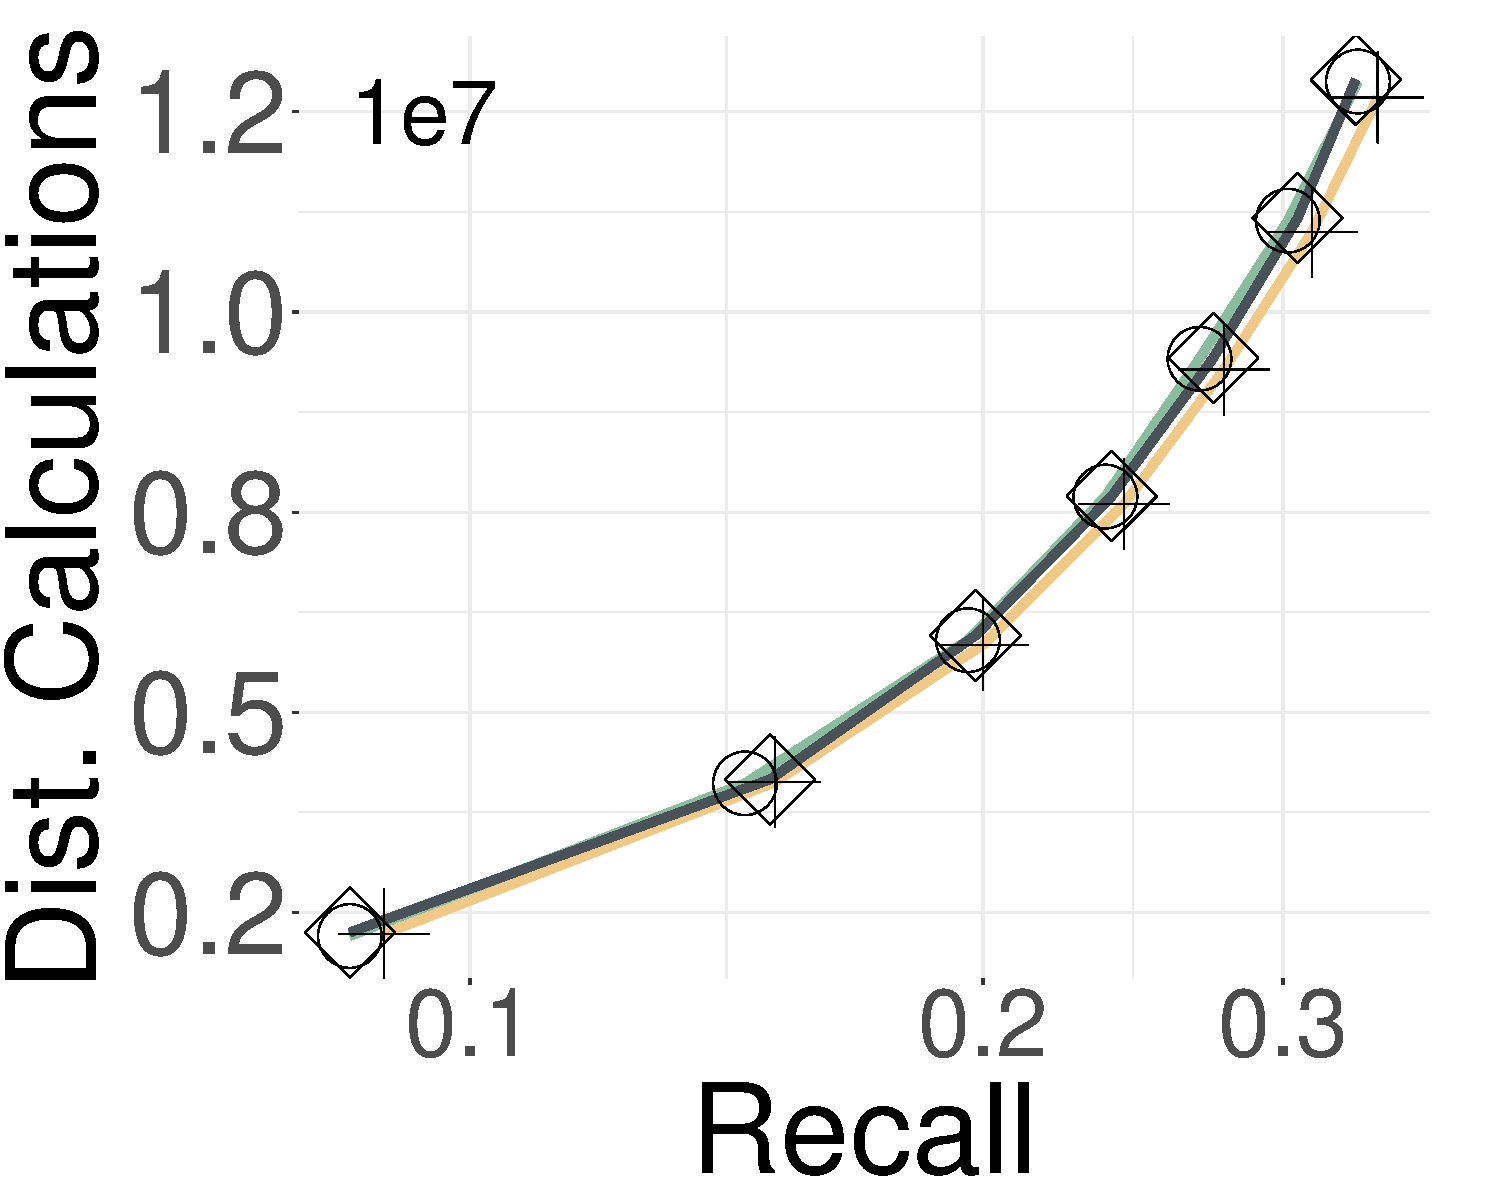
\includegraphics[width=\textwidth]{../img/Experiments/RNG/DC_POW1.pdf}
		\caption{{Pow1}}
		\label{fig:RNG:pow1}
		\end{subfigure}	
  \hspace{0.5cm}
    		\begin{subfigure}{0.28\columnwidth}
			\centering
			\captionsetup{justification=centering}	
				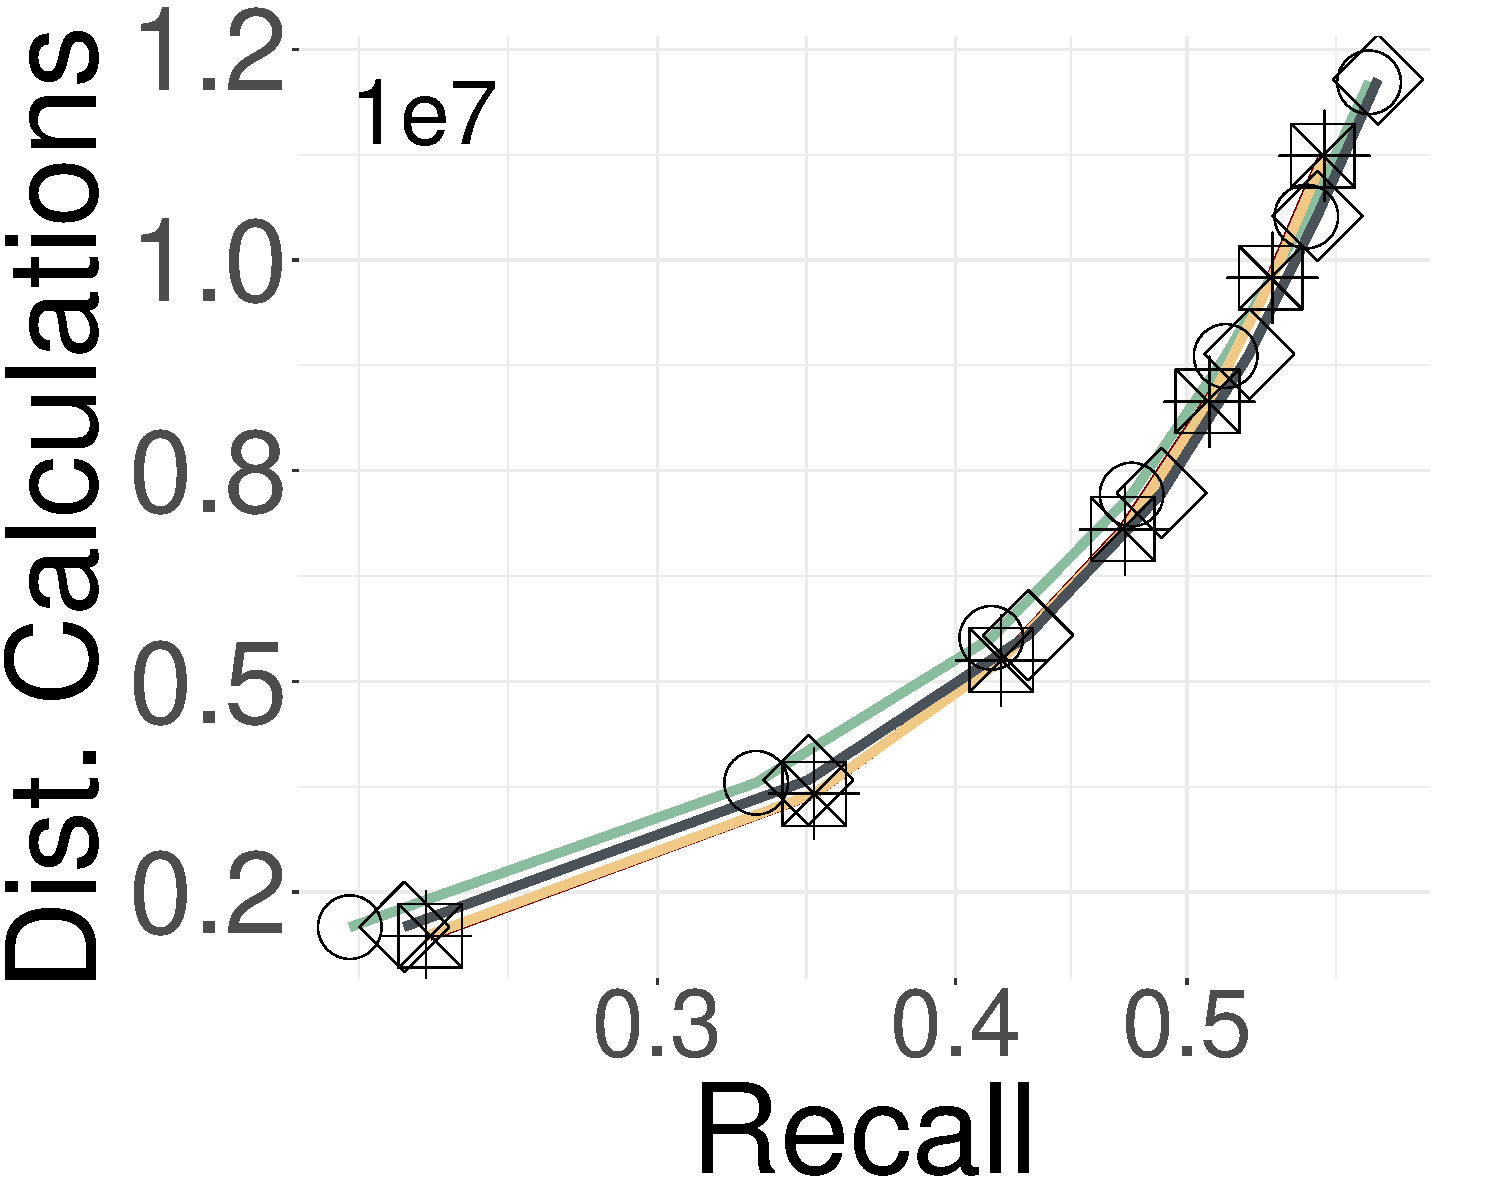
\includegraphics[width=\textwidth]{../img/Experiments/RNG/DC_POW5n.pdf}
		\caption{{Pow5}}
		\label{fig:RNG:deep100GB}
		\end{subfigure}	
  \hspace{0.5cm}
		\begin{subfigure}{0.28\columnwidth}
			\centering
			\captionsetup{justification=centering}	
				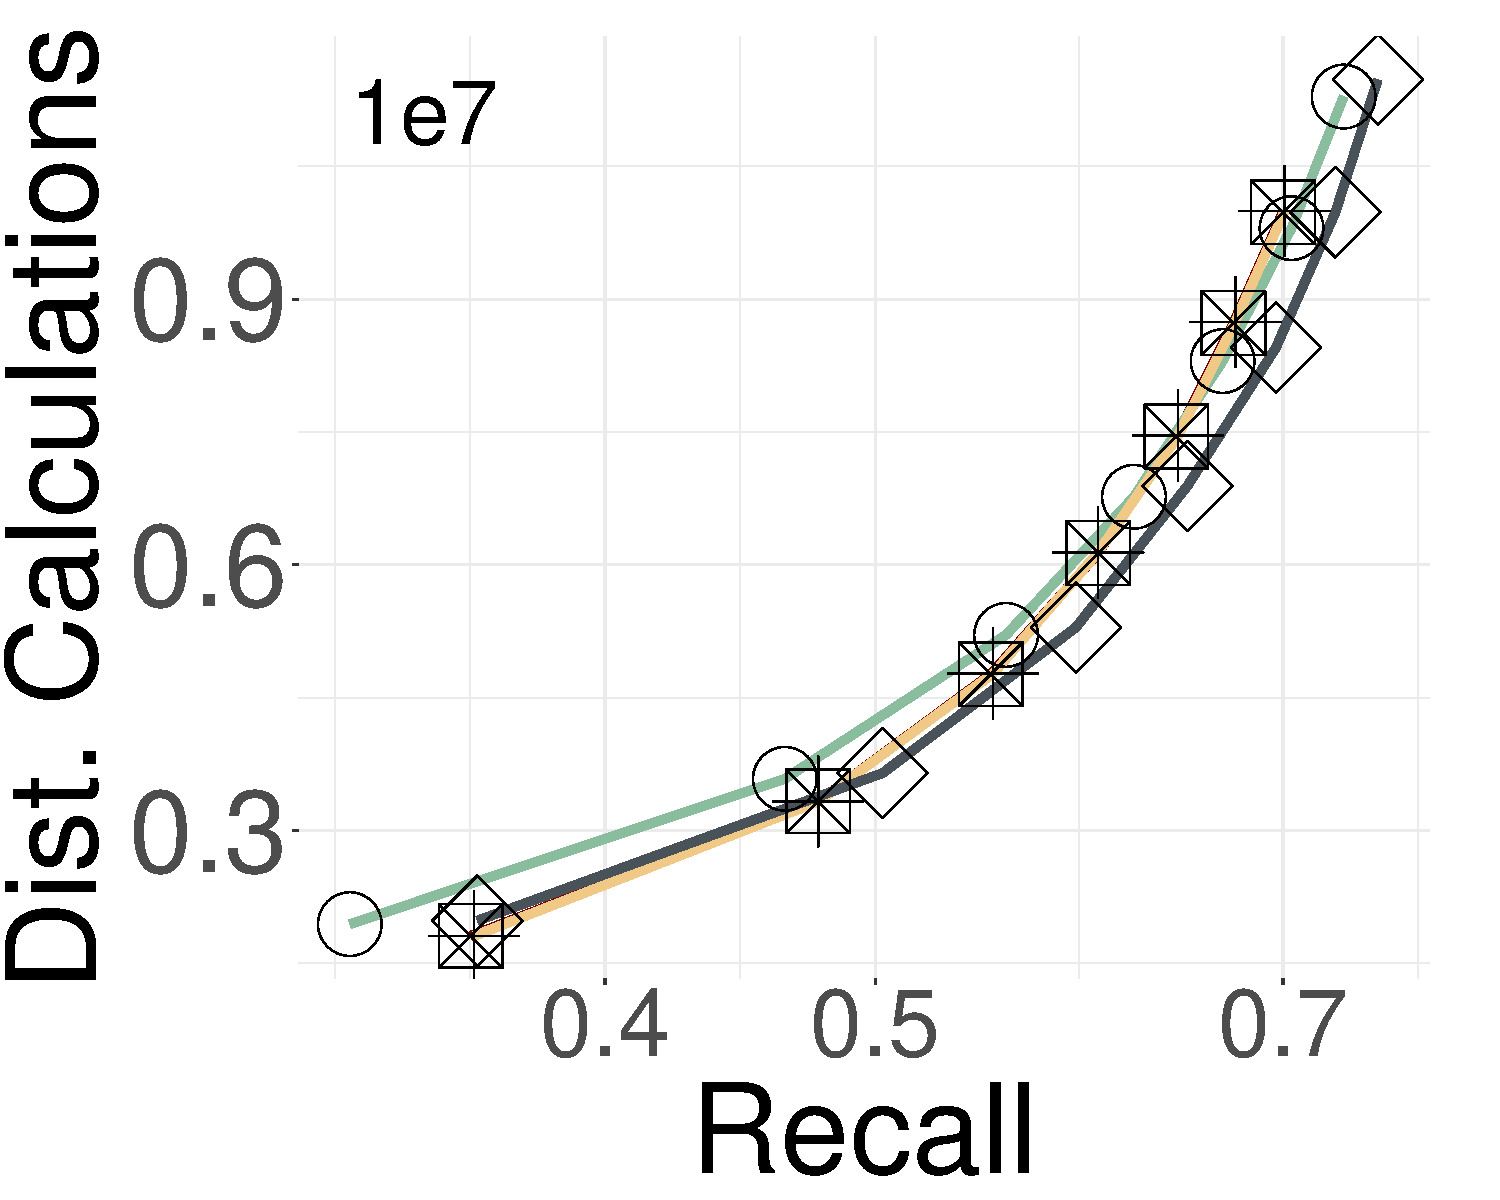
\includegraphics[width=\textwidth]{../img/Experiments/RNG/DC_POW50n.pdf}
		\caption{{Pow50}}
		\label{fig:RNG:pow50}	
  \end{subfigure}	
		\caption{{ND methods performance on random datasets}}
		\label{fig:RNG:search:pow}

 \end{figure}

\subsection{Seed Selection}
In this set of experiments, we evaluate four of the most frequently used Seed Selection (SS) strategies for the beam search algorithm: SN~\cite{hnsw,elpis}, MD~\cite{nsg,vamana}, KS~\cite{kgraph,nsw11,dpg,vamana,nssg}, and KD~\cite{efanna,SPTAG1,hcnng} (note that KM and LSH are excluded as they are not commonly used in graph-based methods). We also include the baseline method SF, which, while not previously applied in the literature, serves as a reference. Each SS strategy is tested using the same graph structure based on Incremental Insertion (II) and RND pruning, which we have identified as the most effective configuration in Section~\ref{subsec:experiments-ND}.

We conduct 100 query experiments for each strategy across the Deep and Sift datasets at sizes of 25GB, 100GB, and 1B. Extrapolating the results to 1M queries, we report the number of distance calculations required to achieve 0.99 recall in Figure~\ref{fig:ss:search}. SN and KS are shown to be the most efficient strategies overall, while SF and MD are the least efficient. The KD strategy demonstrates competitive performance on the 25GB and 100GB datasets, but its performance declines on larger billion-scale datasets. 

KS outperforms SN on smaller datasets (25GB and 100GB); however, this trend reverses on the 1B dataset, where SN becomes more efficient. The difference in distance calculations between SN and KS is approximately 1M on the 25GB dataset and around 10M on the 1B dataset. As the dataset size grows, it becomes necessary to sample more nodes (beyond the beam width used during KS searches) to better represent the dataset and improve the chances of starting the search in a region closer to the query (SN adjusts its sample size logarithmically with dataset size, improving its performance). Figure~\ref{fig:ss:search} also indicates that MD and SF consistently rank among the least efficient strategies, with MD outperforming SF on Deep, but SF surpassing MD on Sift. This suggests that neither MD nor SF is particularly effective or reliable for seed selection.

Next, we analyze how SS strategies affect index construction. We focus on the two best-performing strategies, KS and SN, and study their impact on the same II and RND baseline~\cite{nsw11,dpg,hnsw,nsg,nssg,vamana,elpis,SPTAG1}. These methods are most influenced by the SS strategy, as they use a beam search, which includes seed selection during node insertion.

We build indices using each strategy on the Deep1M and Deep25GB datasets and measure the associated distance calculations. Additionally, we calculate the distance overhead of SN compared to KS, estimating the number of additional 100-NN queries the KS-based graph can answer (with 0.99 recall) before the SN-based graph completes construction.

The results are presented in Table~\ref{tab:ss:idx}. We observe that building the SN-based graph incurs 182 million and 22.3 billion more distance calculations than the KS-based graph on Deep1M and Deep25GB, respectively. Furthermore, the KS-based graph can answer approximately 45K and 1.17 million queries on Deep1M and Deep25GB, respectively, before the SN-based graph finishes its construction.


\newcommand{\sfig}{0.28}
\newcommand{\spbfig}{0.3}

\begin{figure}[htp]
	\captionsetup{justification=centering}
	\centering	
 		\begin{subfigure}{0.018\columnwidth}
			\centering
			\captionsetup{justification=centering}	
			
\includegraphics[width=\textwidth]{img/Experiments/EP/dc.png}
   \vspace{0.18in}
		\end{subfigure}	
		\begin{subfigure}{\sfig\columnwidth}
			\centering
			\captionsetup{justification=centering}	
			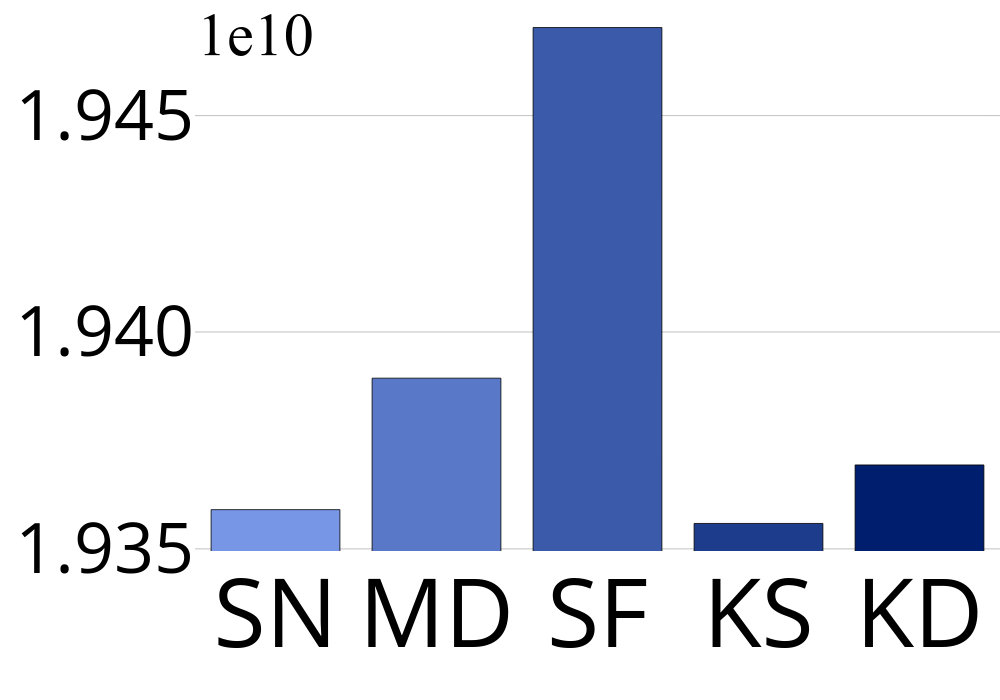
\includegraphics[width=\textwidth]{../img/Experiments/EP/DEEP_25GB_100.png}
		\caption{{Deep25GB}}
		\label{fig:ss:deep1b}
		\end{subfigure}	
	%	\captionsetup{justification=centering}
		\begin{subfigure}{\sfig\columnwidth}
			\centering
			\captionsetup{justification=centering}	
			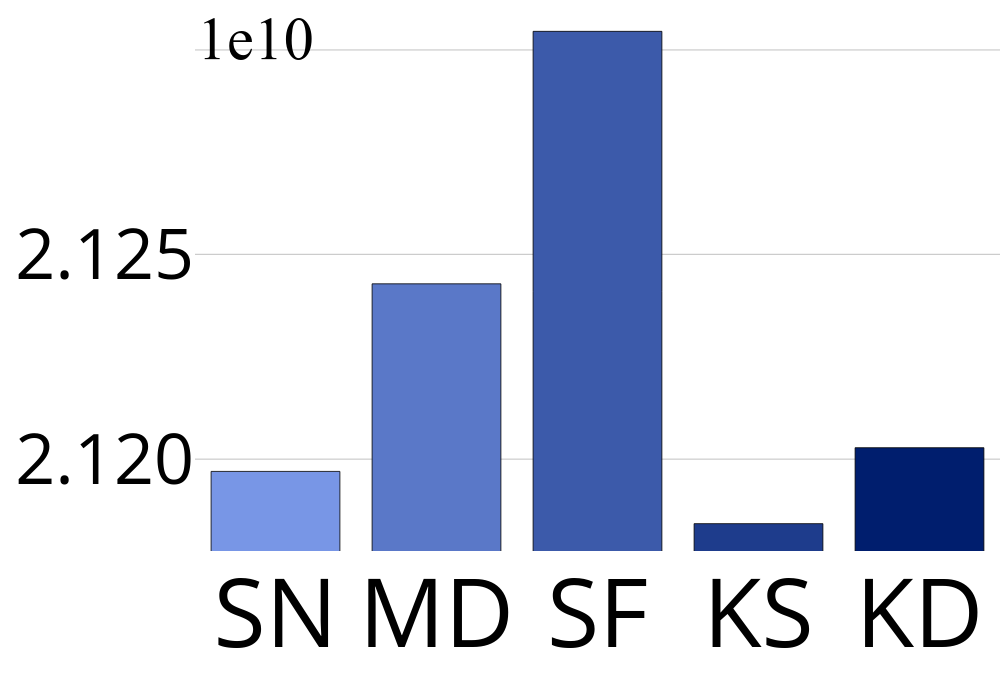
\includegraphics[width=\textwidth]{../img/Experiments/EP/DEEP_100GB_100.png}
		\caption{{Deep100GB}}
		\label{fig:ss:deep1b}
		\end{subfigure}		
		\begin{subfigure}{\sfig\columnwidth}
			\centering
			\captionsetup{justification=centering}	
			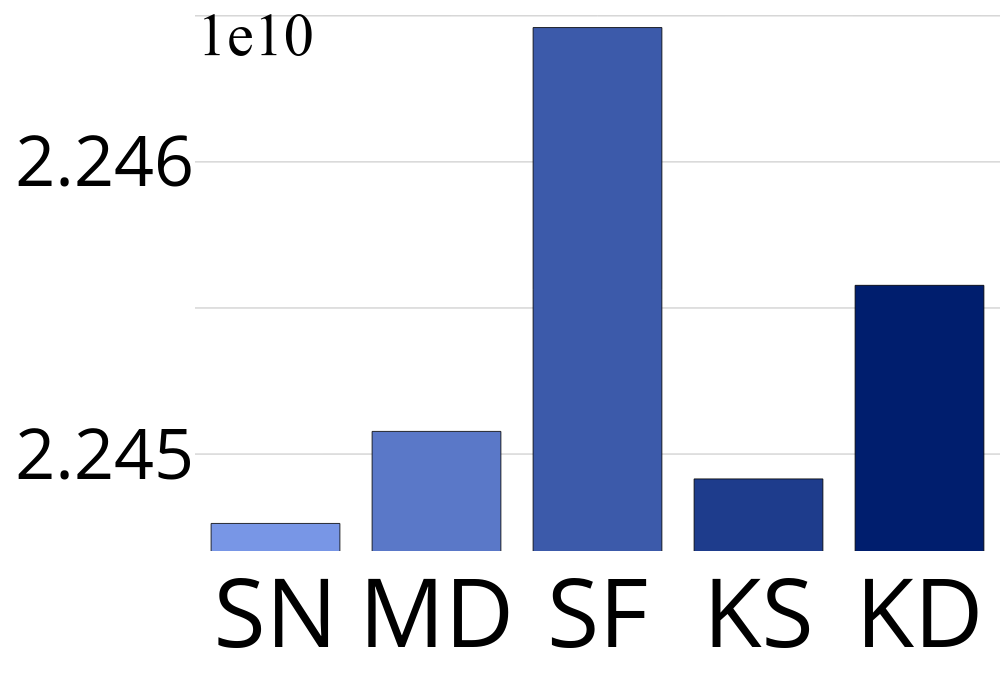
\includegraphics[width=\textwidth]{../img/Experiments/EP/DEEP_1B_100.png}
		\caption{{Deep1B}}
		\label{fig:ss:deep1b}
		\end{subfigure}	

	\begin{subfigure}{0.018\columnwidth}
			\centering
			\captionsetup{justification=centering}	
			
\includegraphics[width=\textwidth]{img/Experiments/EP/dc.png}
   \vspace{0.2in}
		\end{subfigure}	
		\begin{subfigure}{\sfig\columnwidth}
			\centering
			\captionsetup{justification=centering}	
			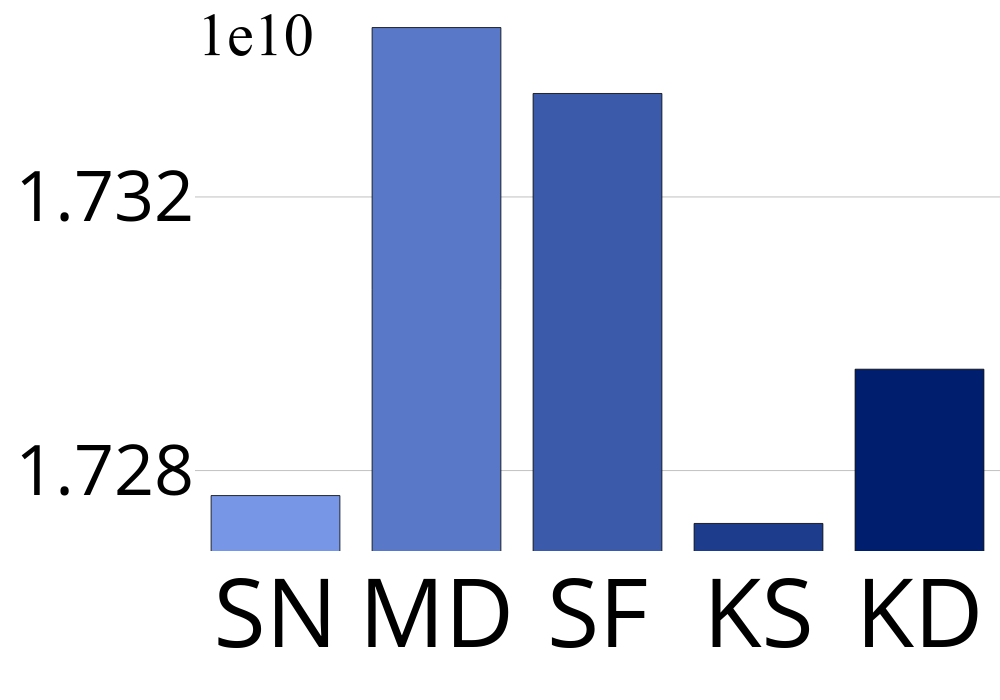
\includegraphics[width=\textwidth]{../img/Experiments/EP/SIFT_25GB_100.png}
		\caption{{Sift25GB}}
		\label{fig:ss:sift1b}
		\end{subfigure}	
	%	\captionsetup{justification=centering}
		\begin{subfigure}{\sfig\columnwidth}
			\centering
			\captionsetup{justification=centering}	
			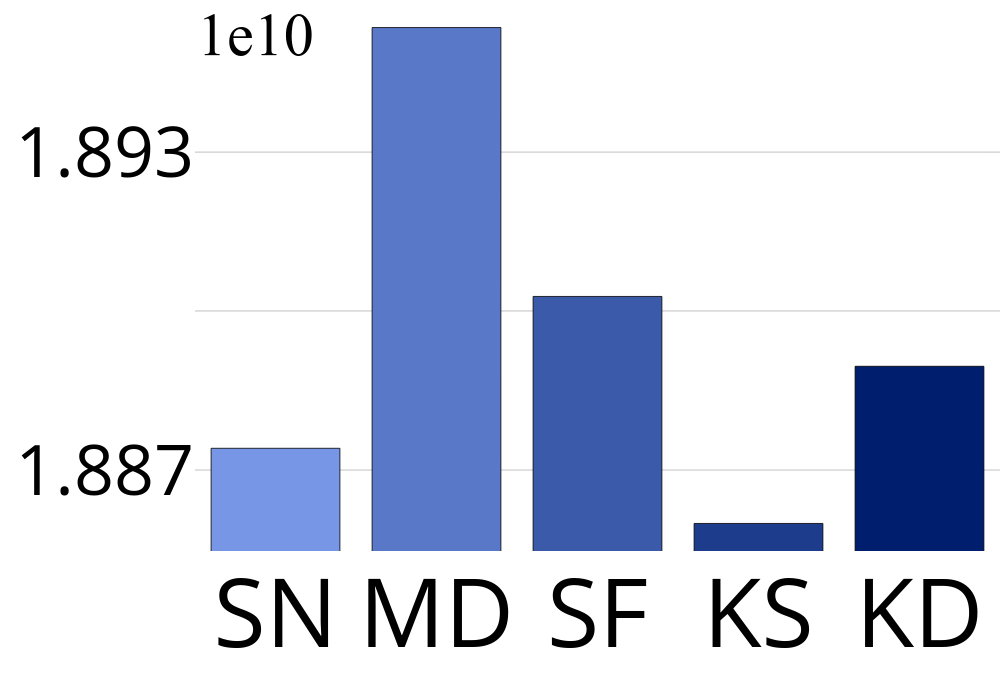
\includegraphics[width=\textwidth]{../img/Experiments/EP/SIFT_100GB_100.png}
		\caption{{Sift100GB}}
		\label{fig:ss:sift1b}
		\end{subfigure}		
		\begin{subfigure}{\sfig\columnwidth}
			\centering
			\captionsetup{justification=centering}	
			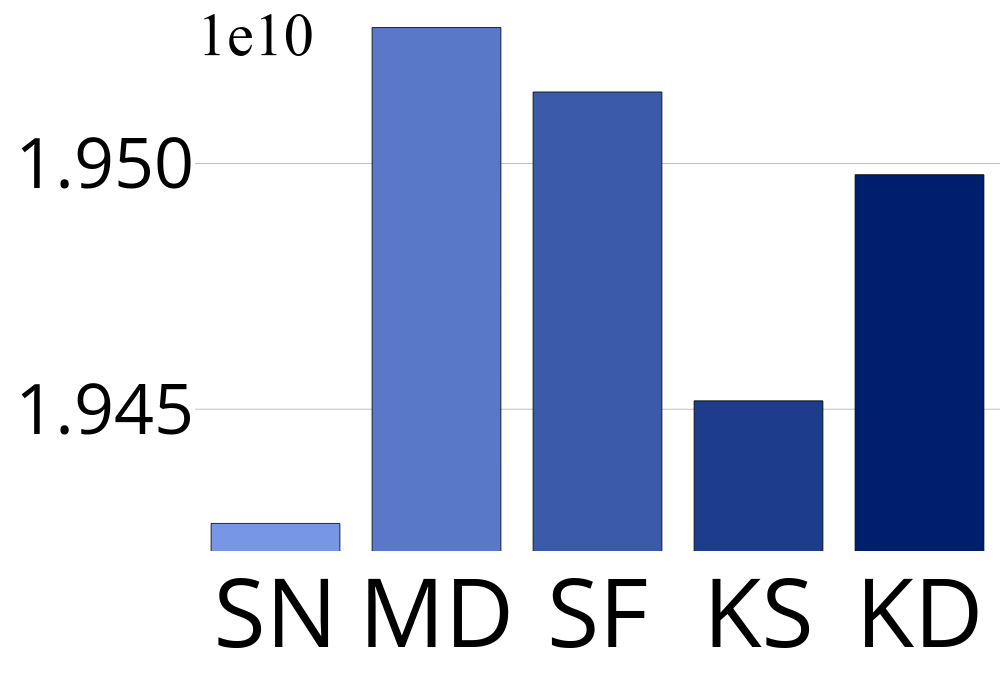
\includegraphics[width=\textwidth]{../img/Experiments/EP/SIFT_1B_100.png}
		\caption{{Sift1B}}
		\label{fig:ss:sift1b}
		\end{subfigure}	
\caption{The impact of SS Methods on Query Answering}
\label{fig:ss:search}
 \end{figure}
 


\begin{table}[h!]
\centering
\begin{tabular}{@{}lcc@{}}
\toprule
%\textbf{Metric} 
& \textbf{Deep1M} & \textbf{Deep25GB} \\ 
\midrule
\textbf{Dist. Calculations (SN)} & 4.3 billion & 1.49 trillion \\
\textbf{Dist. Calculations (KS)} & 4.1 billion & 1.46 trillion \\
\midrule
\textbf{Overhead (SN vs. KS)} & 182 million & 22.3 billion \\
\textbf{Additional Queries} & 44,959 & 1,165,870 \\
\bottomrule
\end{tabular}
\caption{The impact of SS methods on Indexing Performance}
\label{tab:ss:idx}
\end{table}

\begin{comment}
    \subsection{Empirical Analysis of the theoretical complexity of Beam search}
\ilias{I have added this subsection to appendix, i think it's better to have it there with also proof of approximations between the NDs approaches}
Beam search, introduced by Raj Reddy in 1977, is a core algorithm widely used across various fields, including speech recognition, machine translation, and natural language processing. It operates by exploring a restricted number of hypotheses, referred to as the "beam," improving efficiency compared to exhaustive search approaches. However, beam search trades off completeness and optimality for speed, as it may prune potential goal states, and thus does not always guarantee finding the best solution. The time complexity of beam search is determined by factors such as the beam width and the maximum allowable path length in the graph. When applied to proximity graphs, as used in spatial data analysis, beam search efficiently explores nearby nodes or edges, making it highly versatile across different domains.

The time complexity of beam search is described by the following formula:

\[
\text{Time Complexity} = O(B \times m \times T) \quad (\text{Eq. 4})
\]

Where \( B \) denotes the beam width, \( m \) represents the average branching factor (or average outdegree in graph search), and \( T \) indicates the maximum path length allowed within the graph. In the worst case, \( T \) is equivalent to the graph's diameter, representing the longest possible path. This formula captures the computational cost of beam search, factoring in the beam width, average outdegree, and graph diameter. However, because the search accuracy for a given beam width is not guaranteed, the exact time complexity can only be approximated by running a search on a query set to determine the necessary beam width for a target accuracy. Sometimes, the differences in beam widths between methods may have a greater impact on time complexity than variations in outdegree or diameter. It is also worth noting that different seed selection strategies can affect time complexity, especially when the number of nearest neighbors required is small.

Below, we provide an analysis of the theoretical time complexity and its alignment with the empirical performance of four state-of-the-art graph-based algorithms. For each method, the graph is built with maximum outdegrees of 40, 40, 50, and 60 for the datasets Deep1M, Deep2M, Deep4M, and Deep8M, respectively. The purpose is to examine how the theoretical time complexity corresponds to the empirical performance of the methods, both in terms of time and the number of distance calculations. All measurements are taken for a target accuracy of 0.99.

\begin{figure}
\centering
\begin{subfigure}{0.45\textwidth}
  \centering
  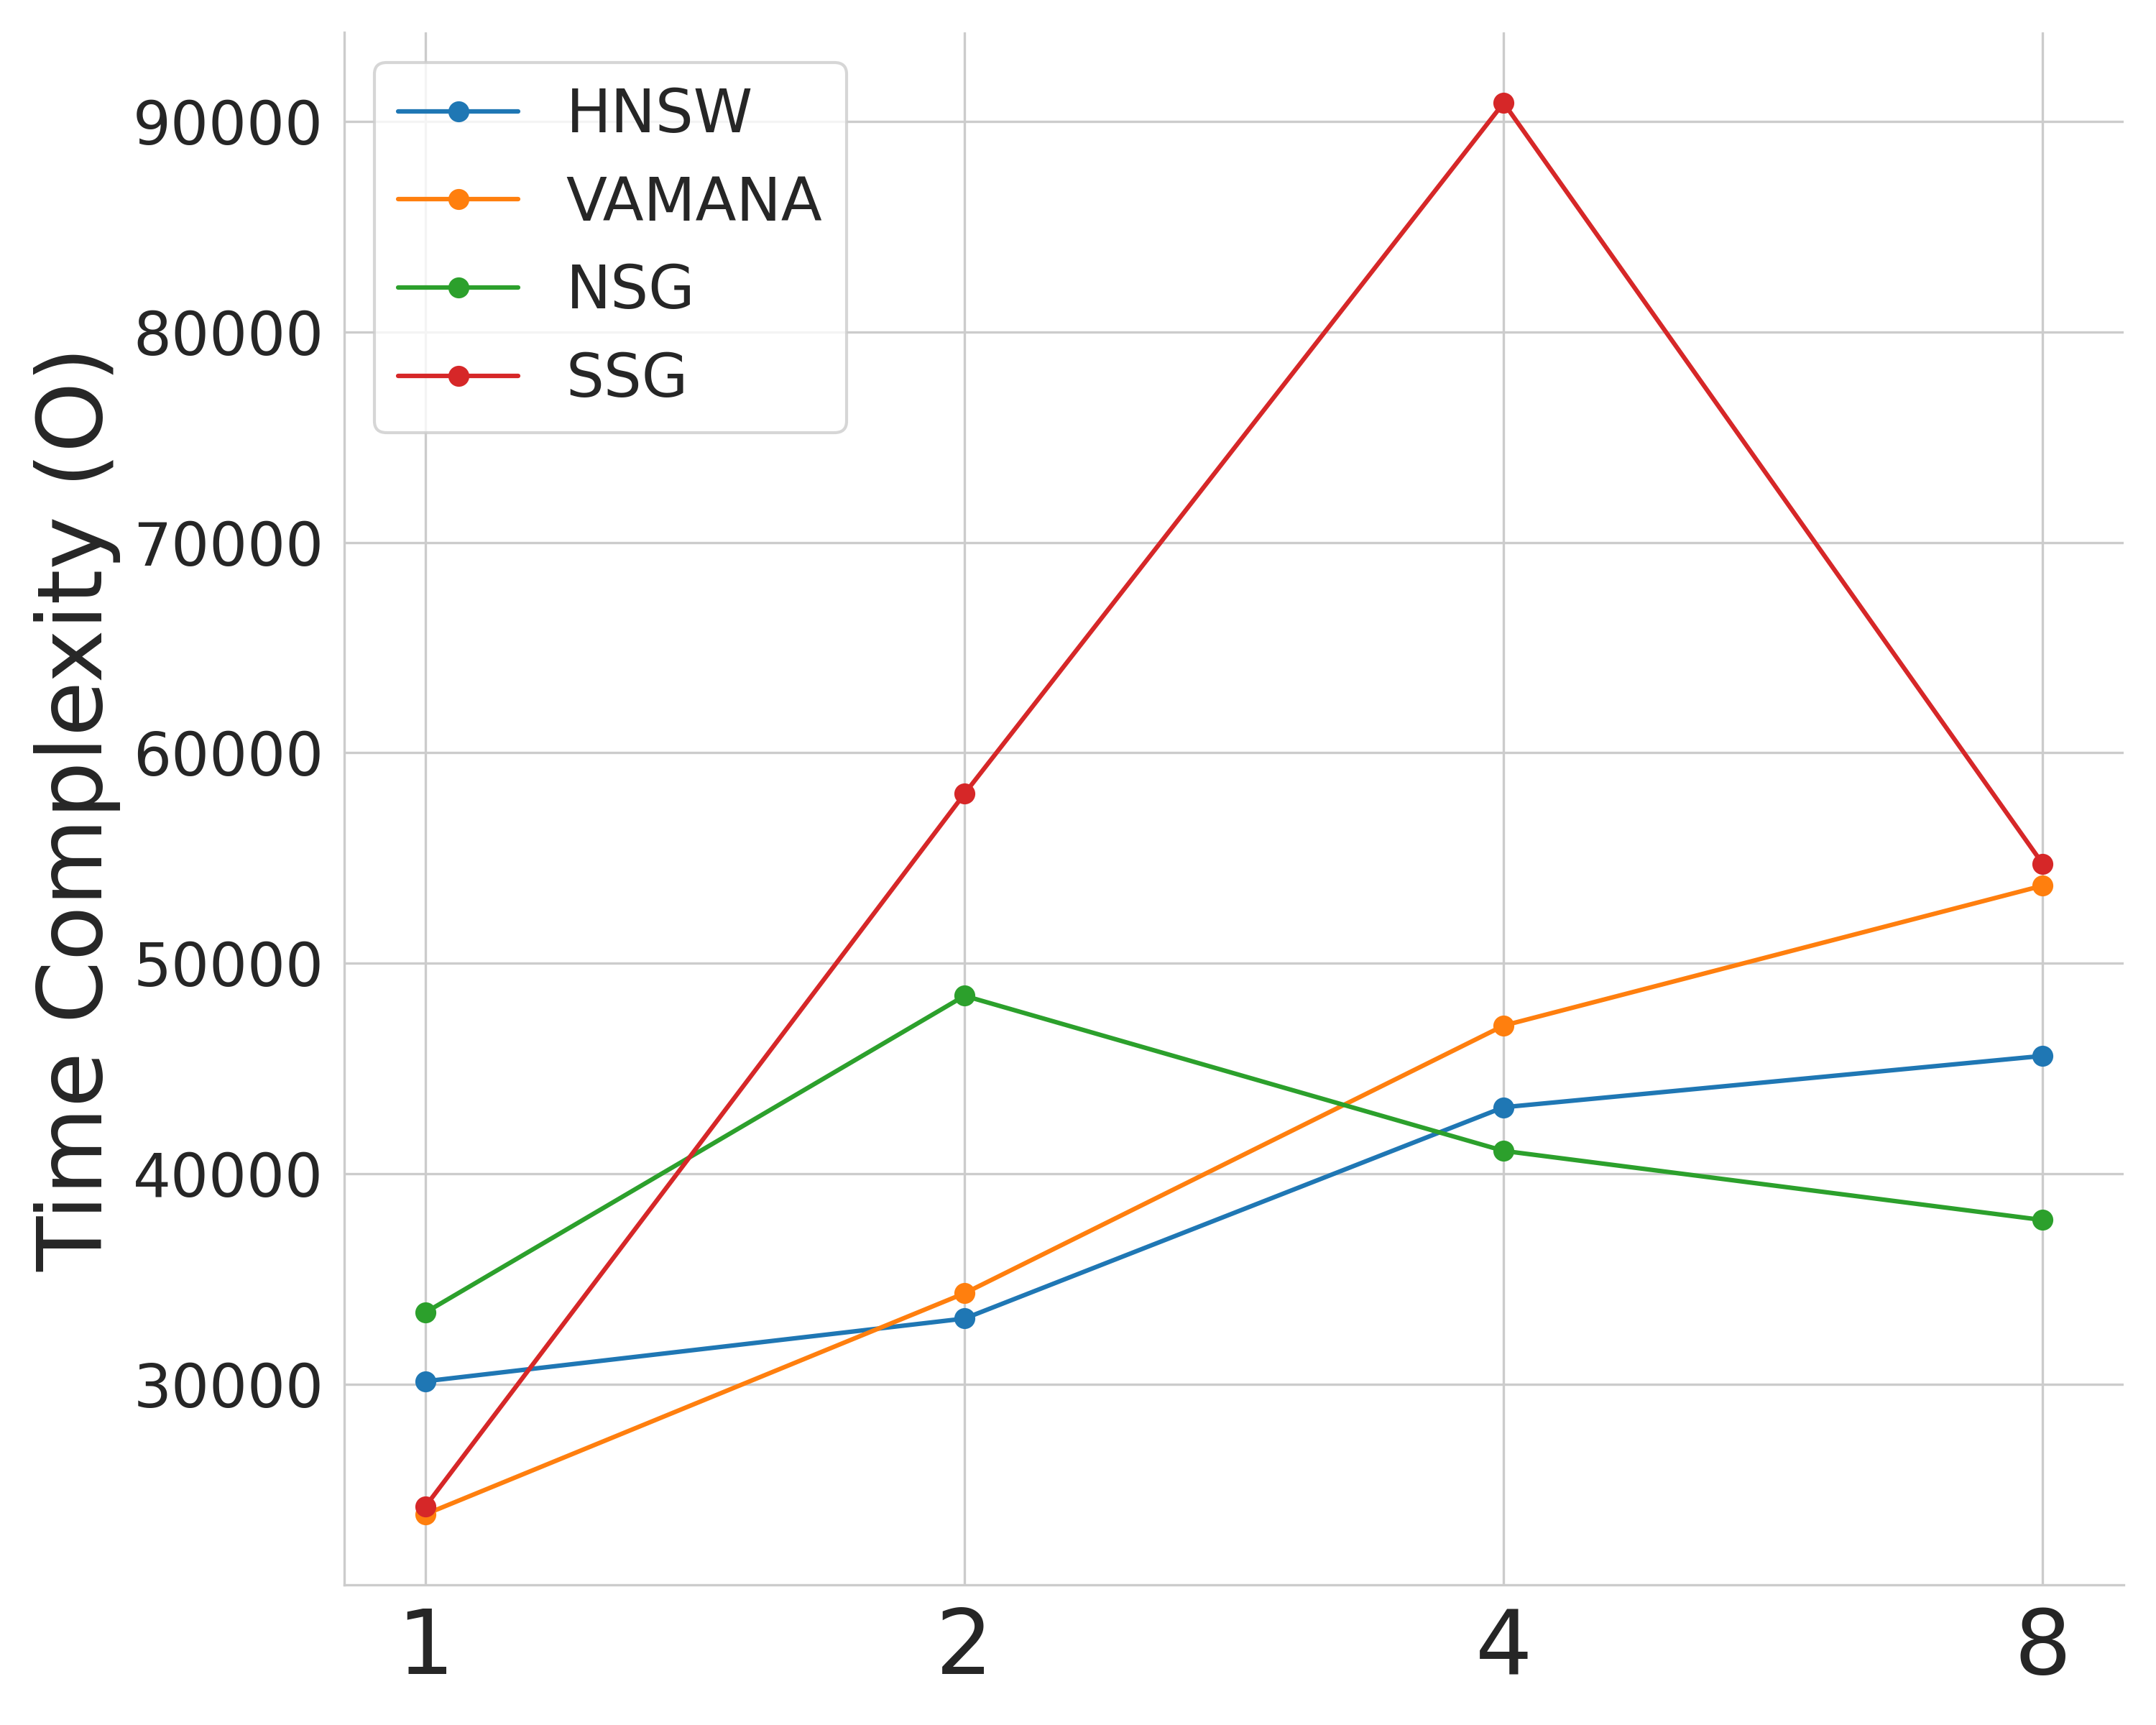
\includegraphics[width=\linewidth]{../img/Experiments/BSC/complexity_size.png}
  \caption{Theoretical Time Complexity}
  \label{fig:cno}
\end{subfigure}
\hfill
\begin{subfigure}{0.45\textwidth}
  \centering
  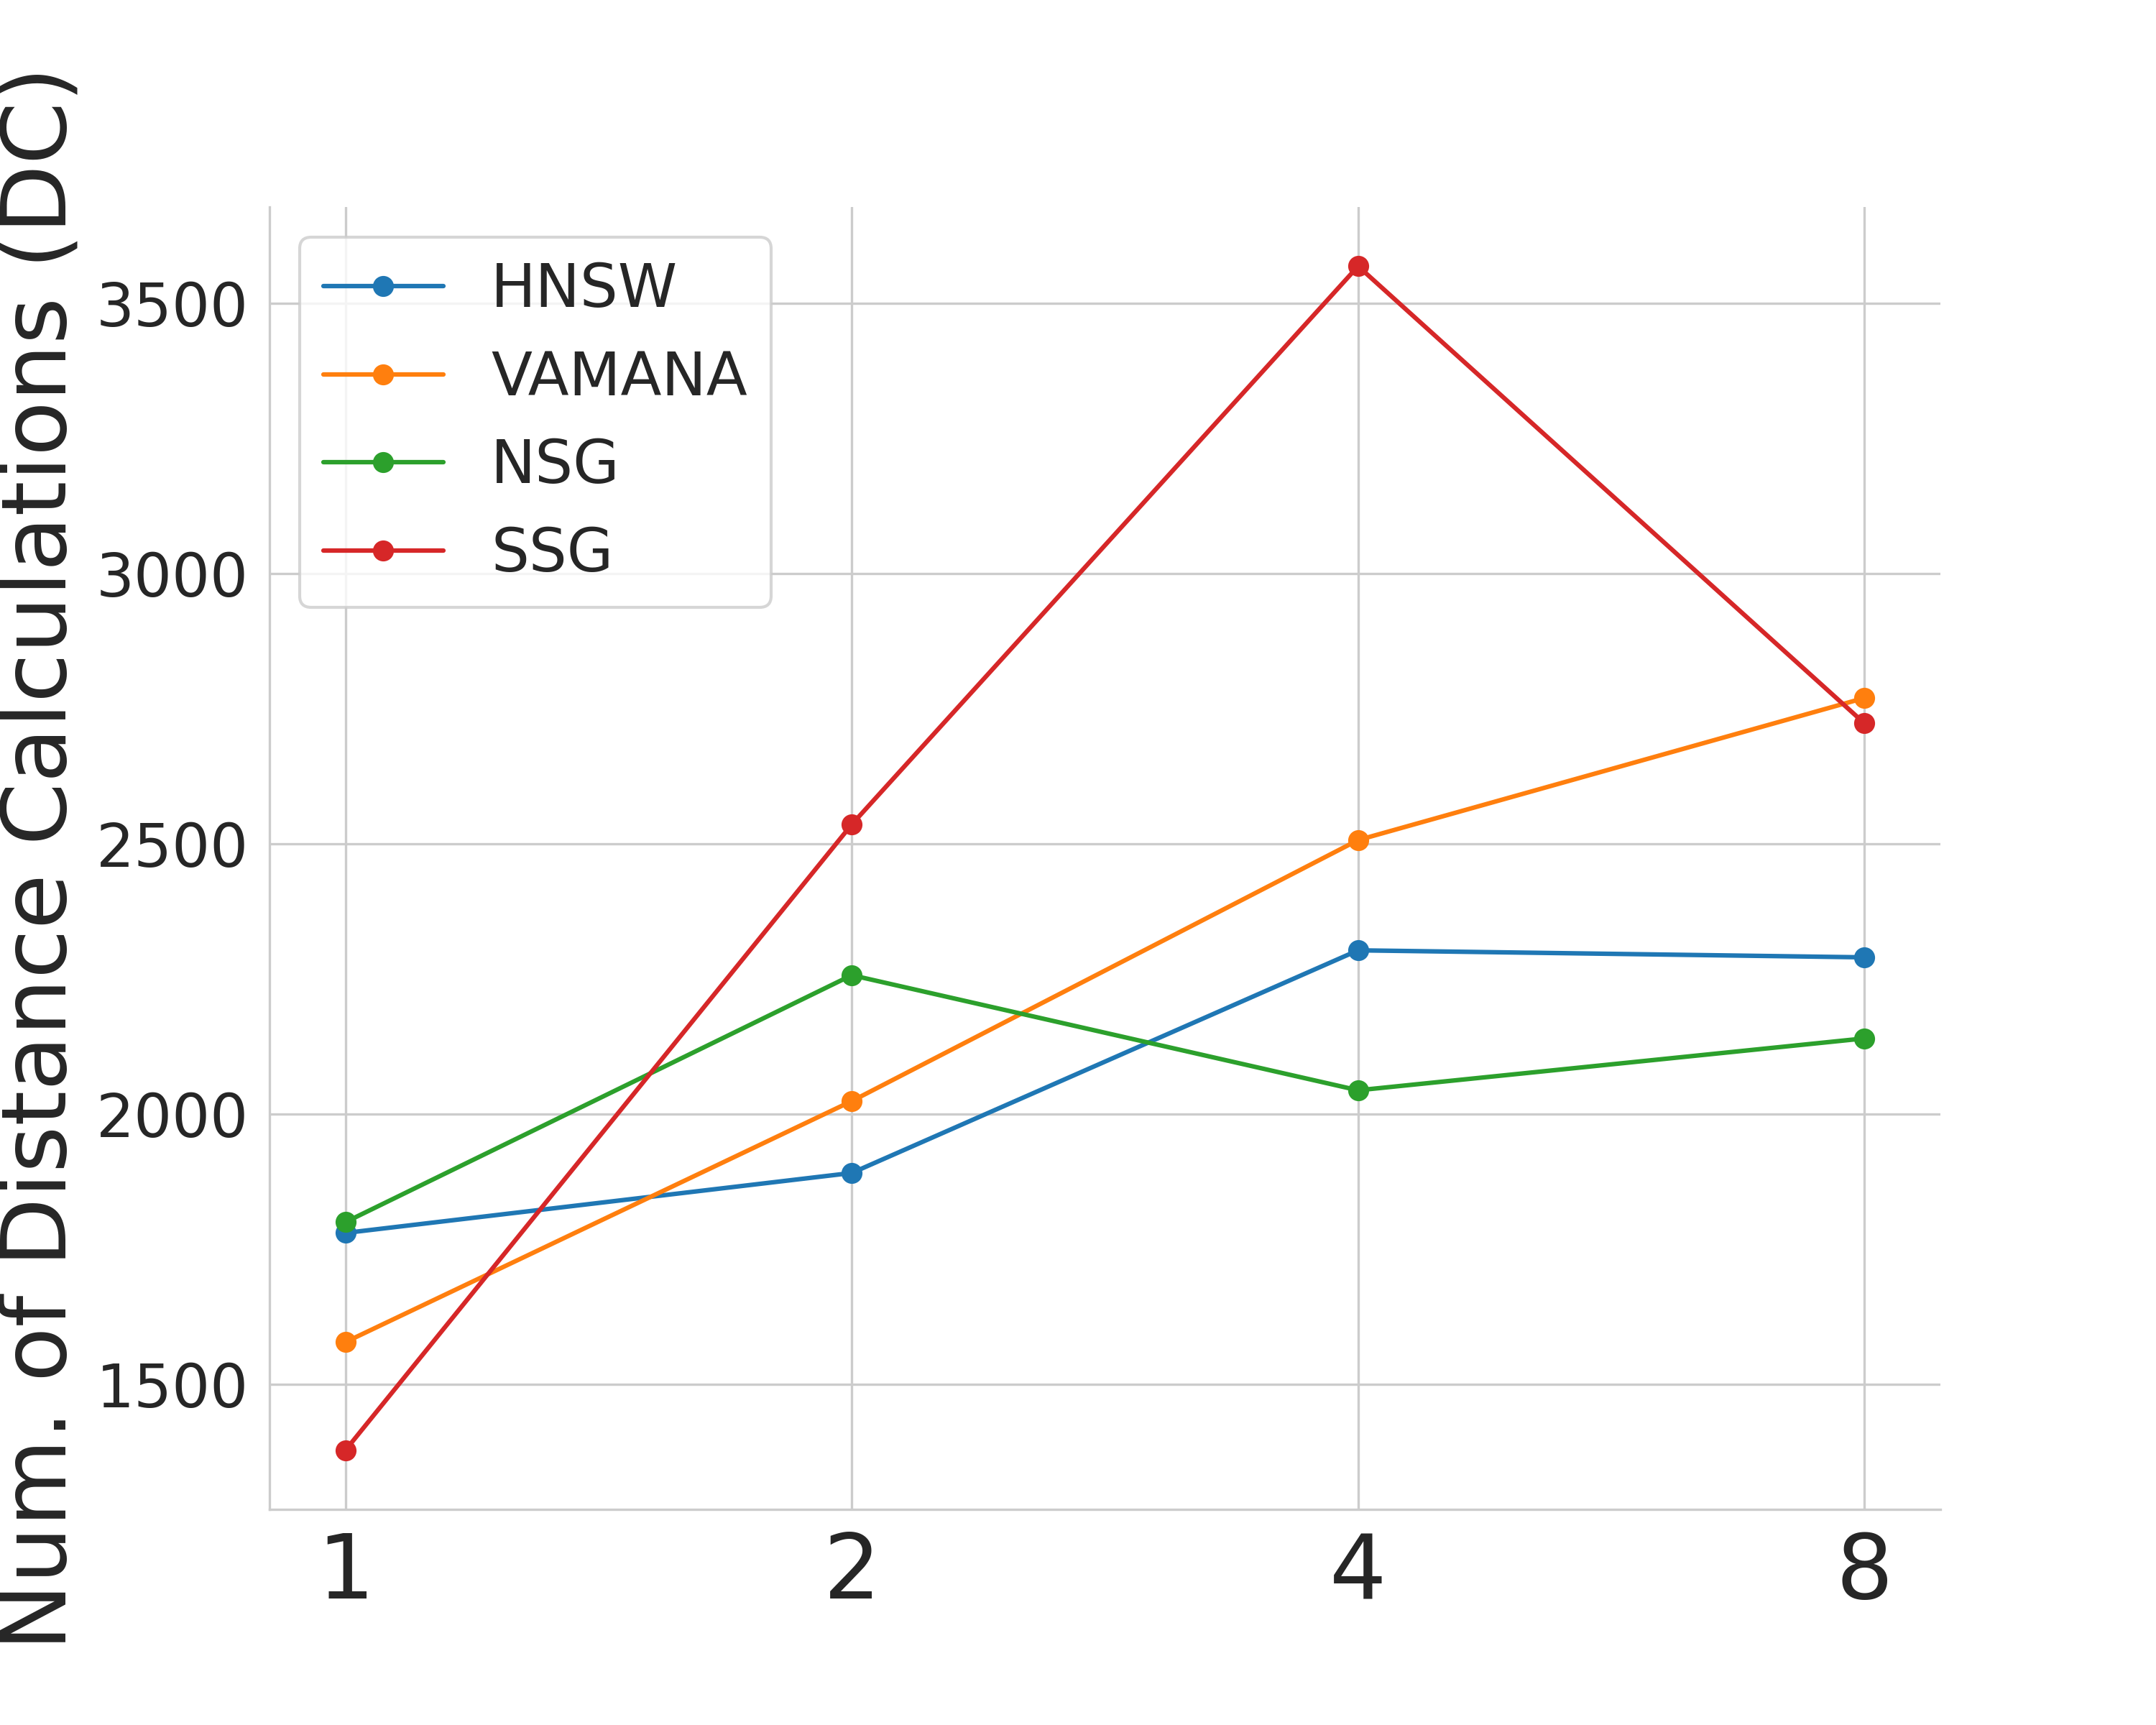
\includegraphics[width=\linewidth]{../img/Experiments/BSC/dc_size.png}
  \caption{Empirical efficiency}
  \label{fig:dc}
\end{subfigure}
\caption{Theoretical and empirical beams search efficiency across different deep1b dataset sizes}
\label{fig:ndc_no_size_plots}
\end{figure}

In Figure ~\ref{fig:ndc_no_size_plots}, we illustrate how the theoretical time complexity of the beam search aligns with the algorithm efficiency, specifically the number of distance calculations across different dataset sizes. As the dataset size increases, we can observe an improvement in the approximation of the empirical complexity (comparing 1M to 2M, 4M, and 8M), as the ranking between methods in terms of beam search efficiency is approximated using the beam search time complexity formula in Eq. 4.
In Figure ~\ref{fig:ndc_no_plots}, we present the comparison between the time complexity and search efficiency of four methods for different deep1b dataset scales.

\begin{figure}[htbp]
\centering
\begin{subfigure}{0.24\textwidth}
  \centering
  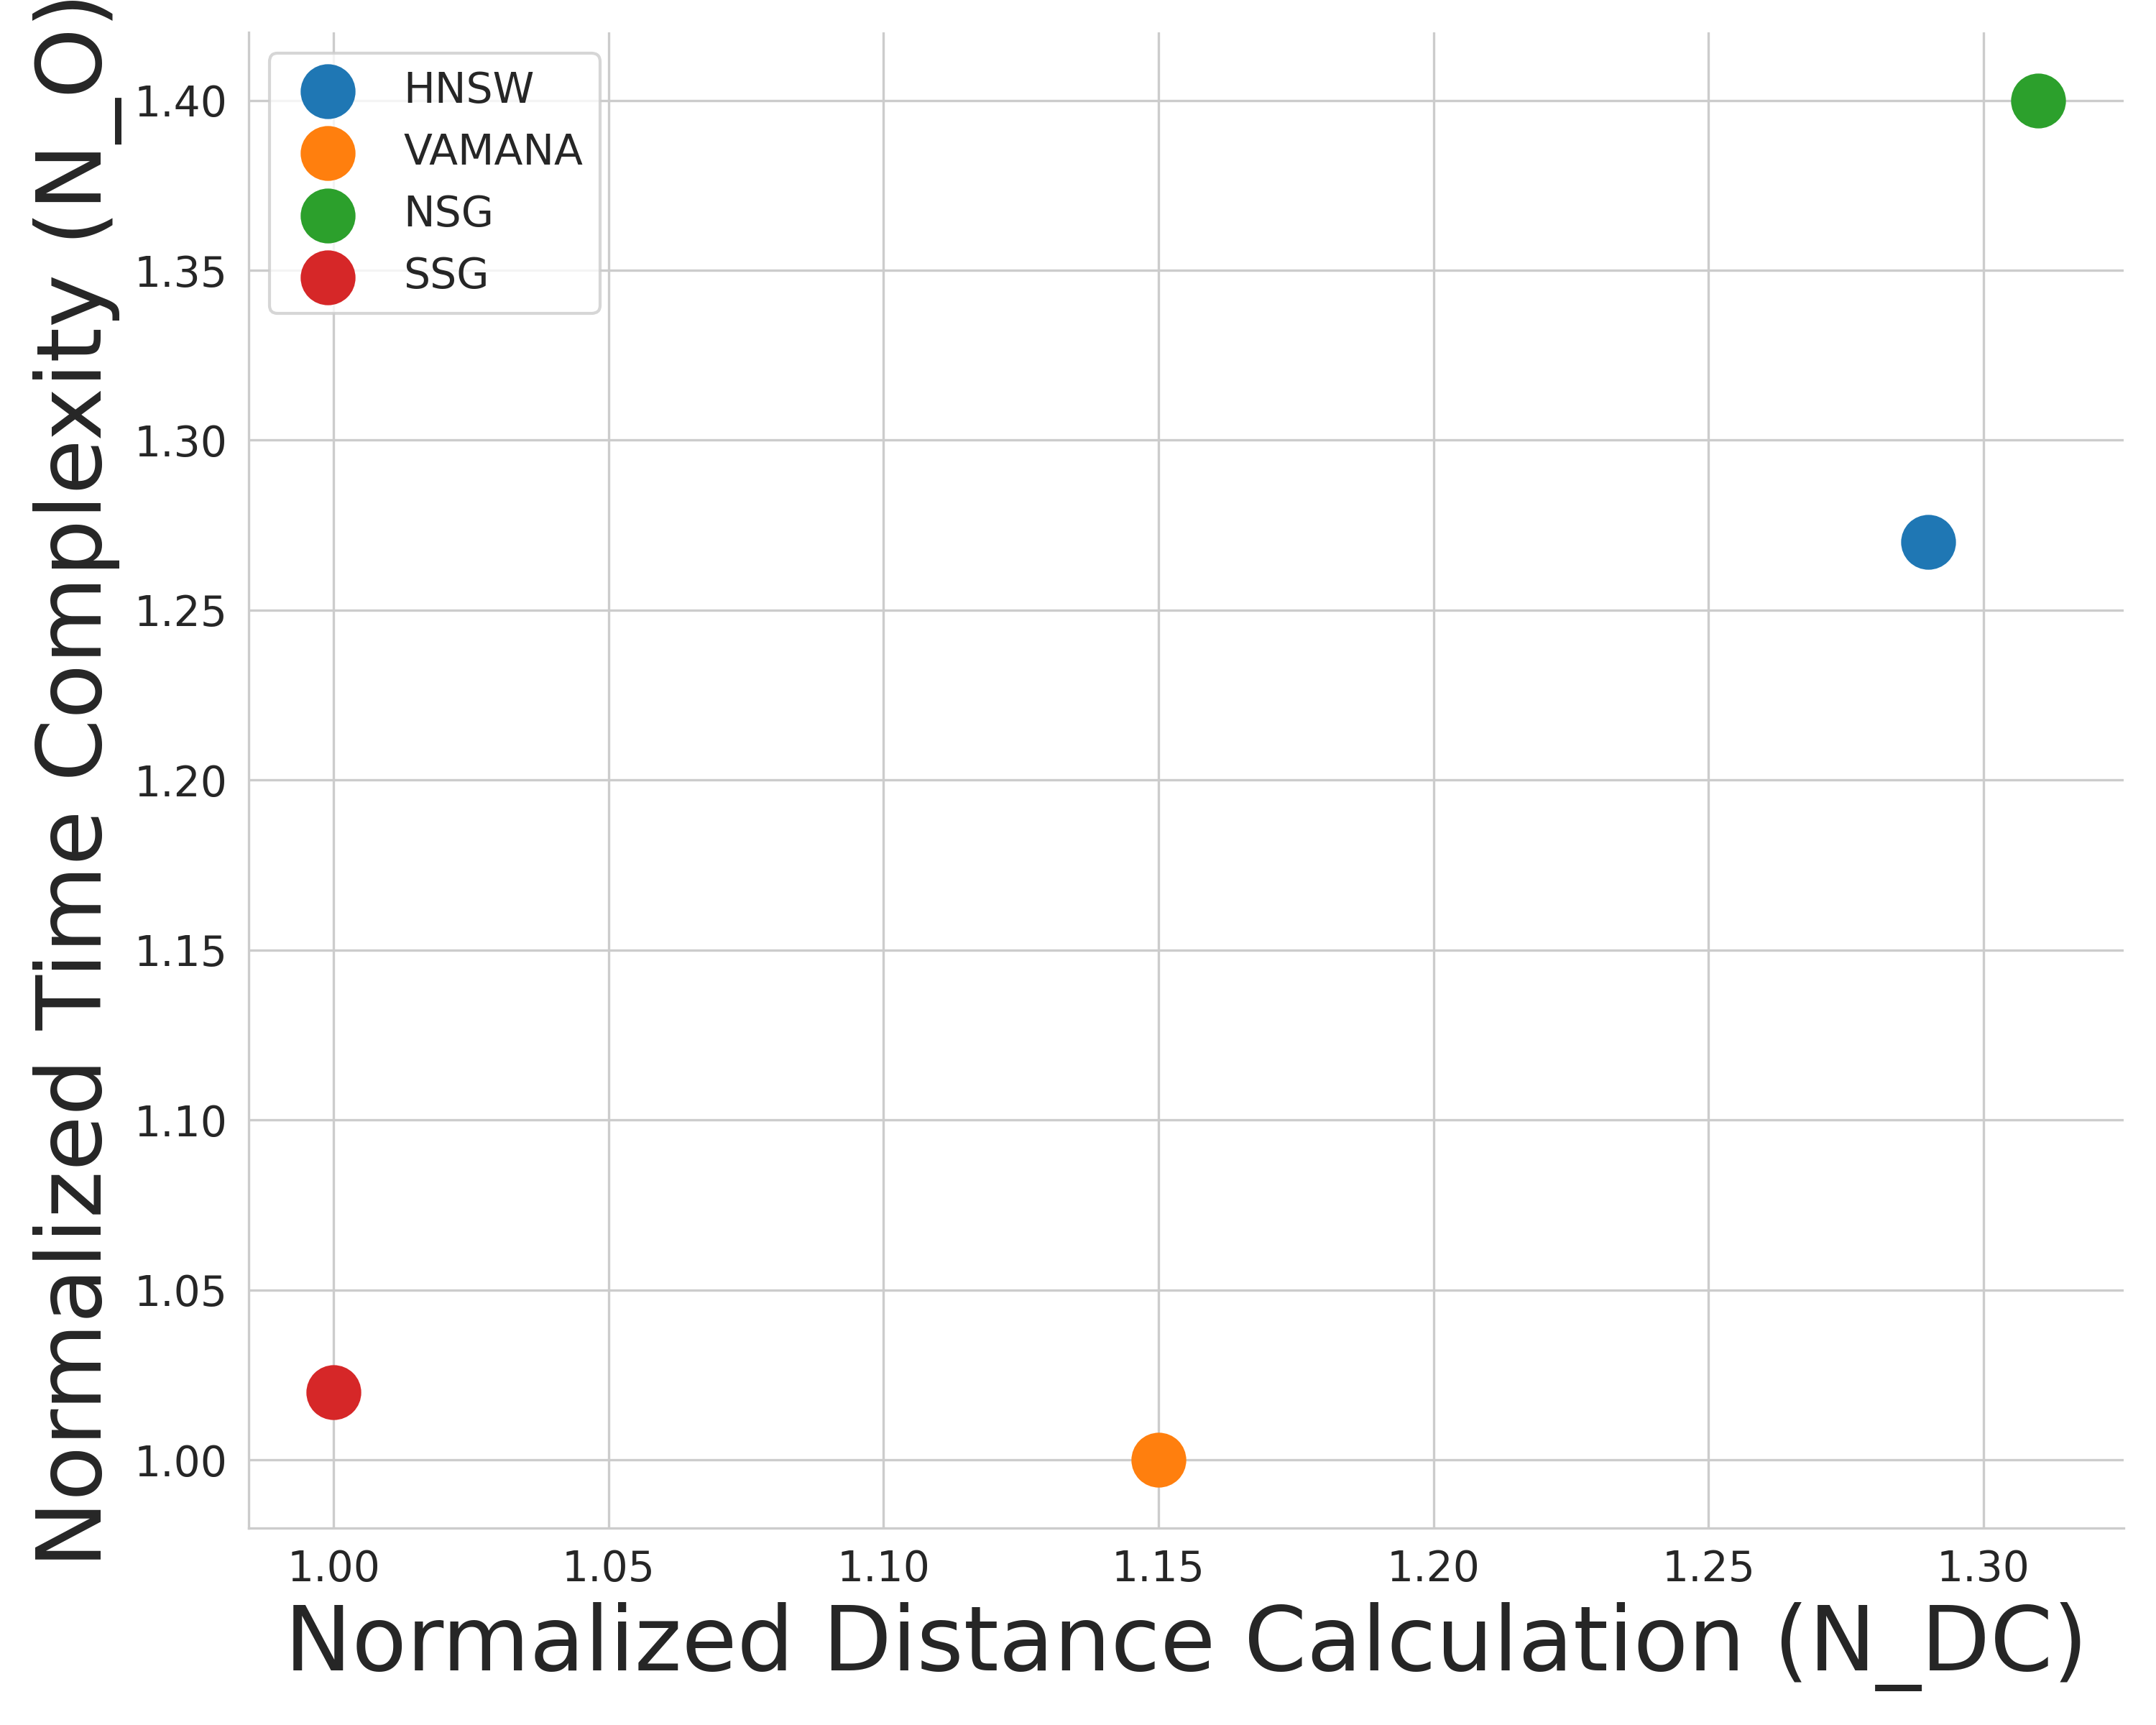
\includegraphics[width=\linewidth]{../img/Experiments/BSC/1_ndc_no.png}
  \caption{Deep1M}
  \label{fig:1_ndc_no}
\end{subfigure}
\hfill
\begin{subfigure}{0.24\textwidth}
  \centering
  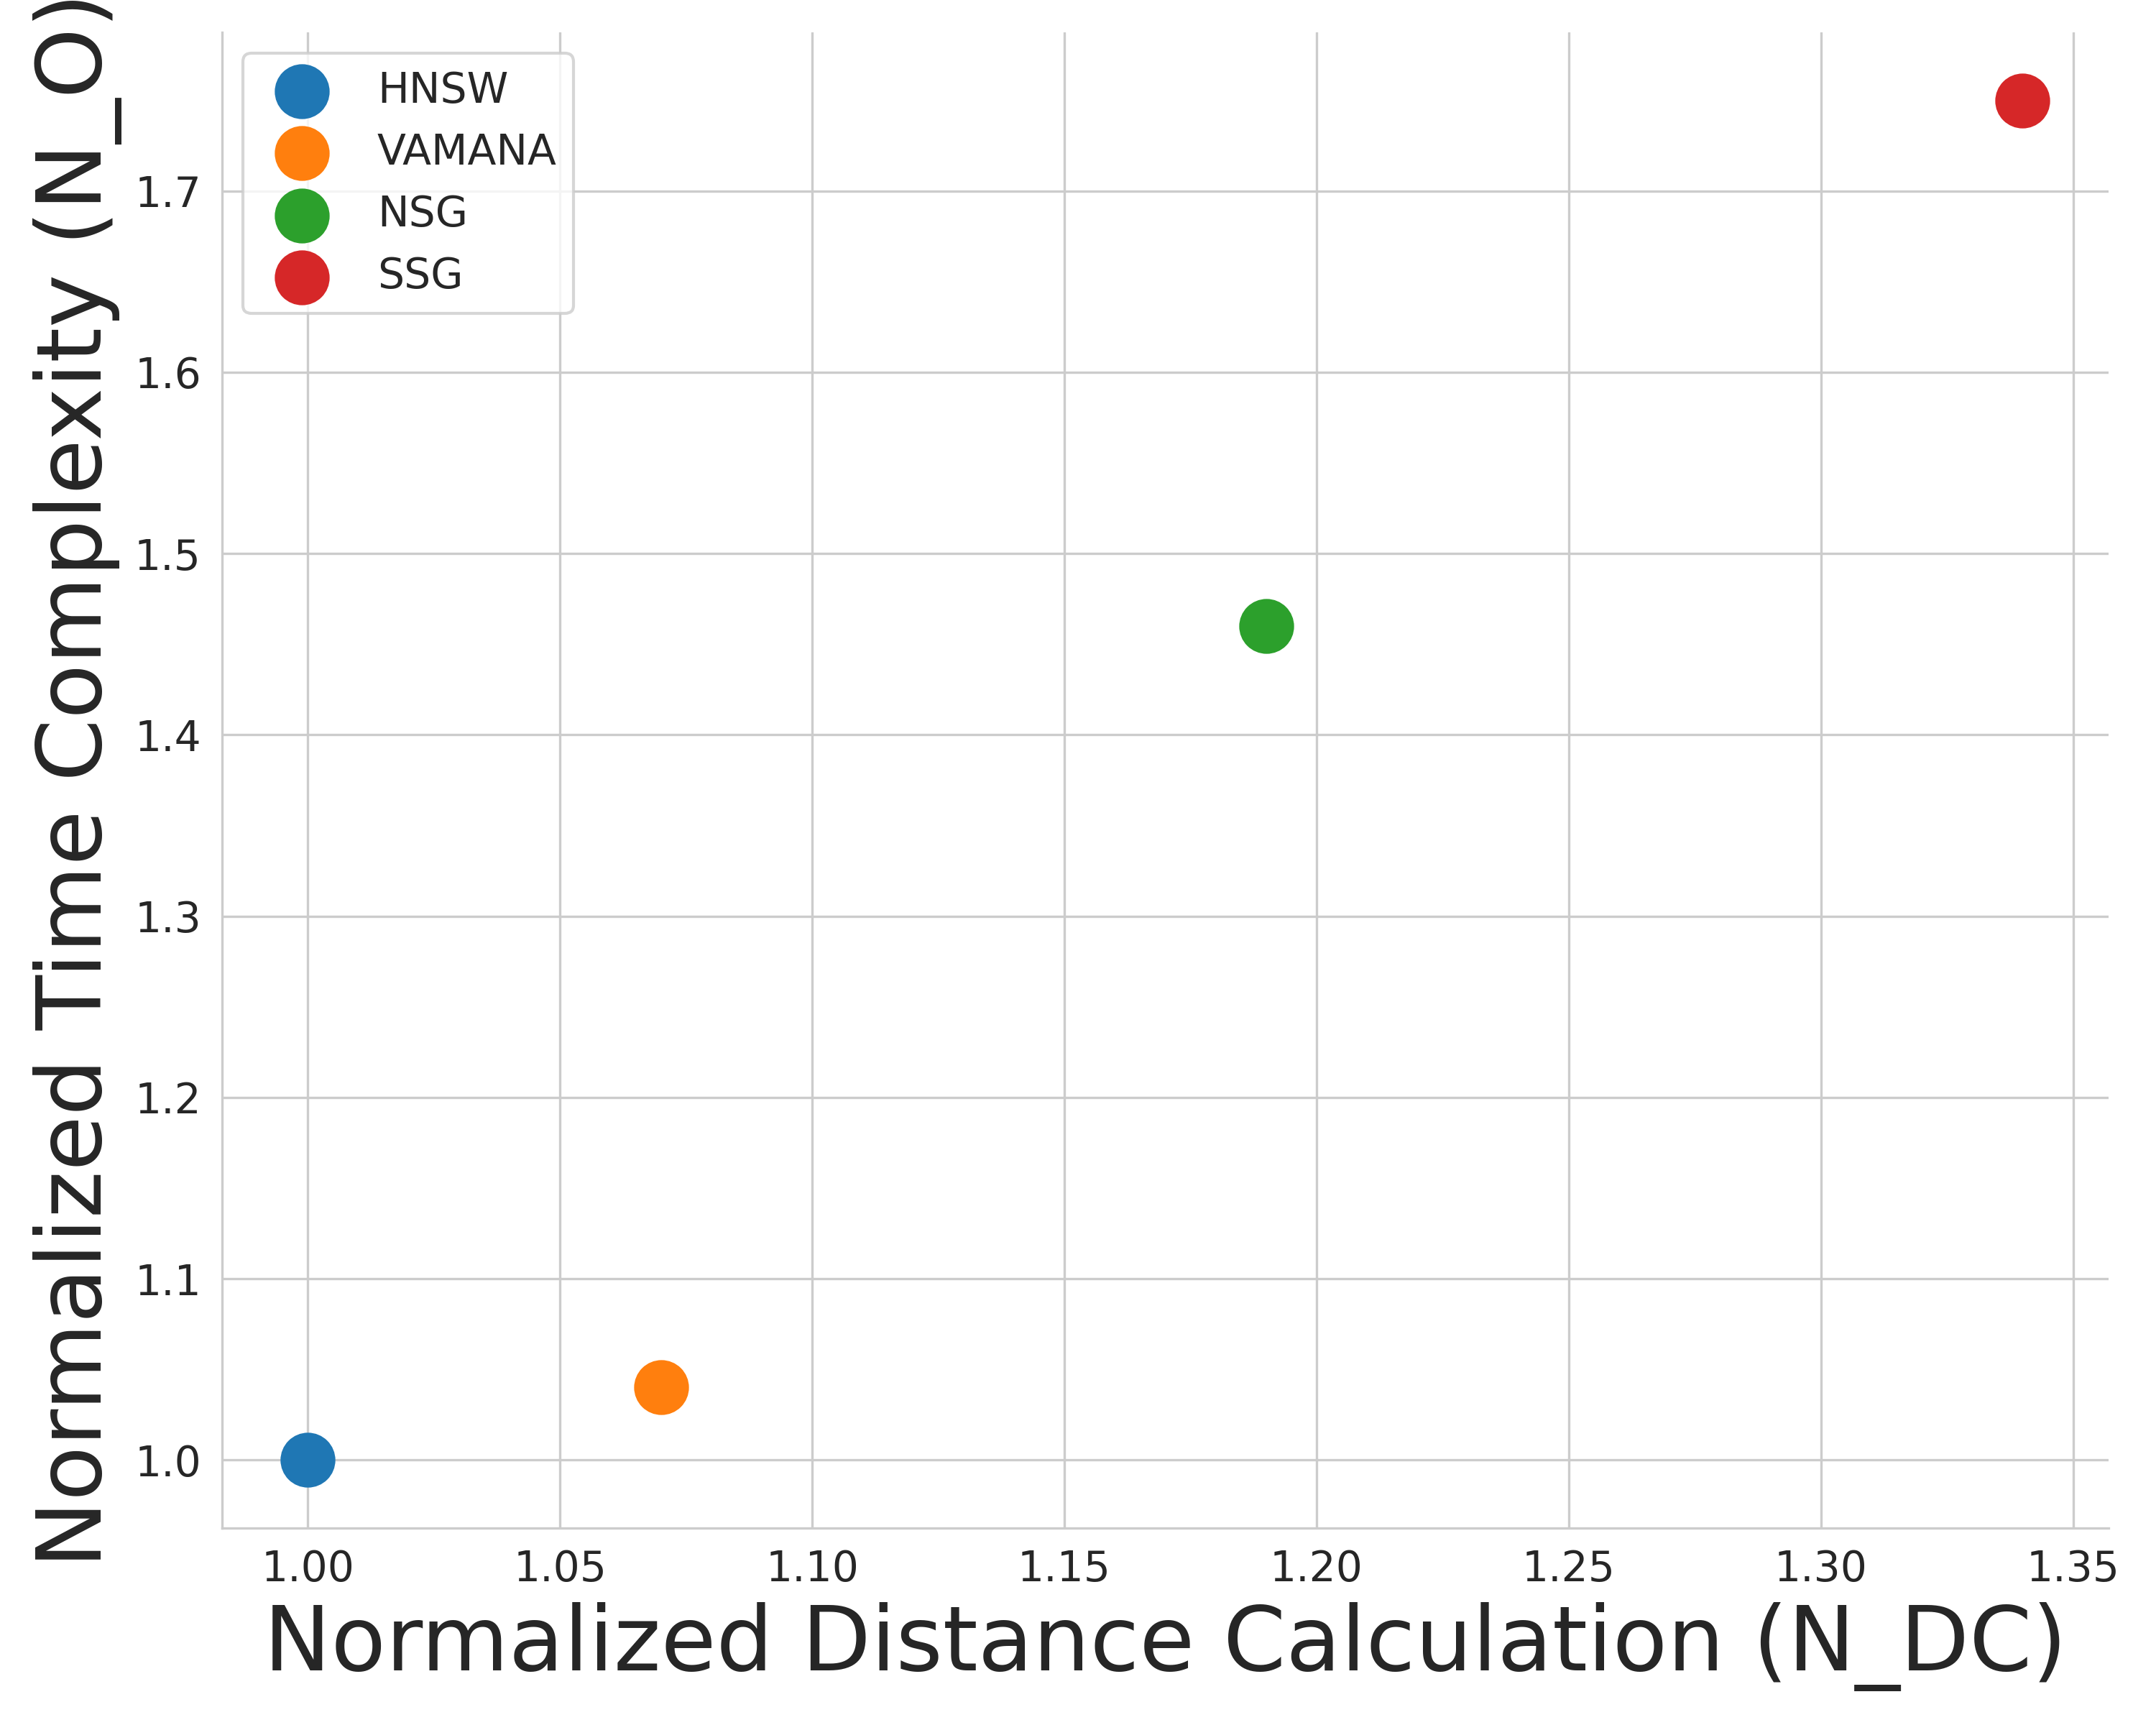
\includegraphics[width=\linewidth]{../img/Experiments/BSC/2_ndc_no.png}
  \caption{Deep2M}
  \label{fig:2_ndc_no}
\end{subfigure}
\begin{subfigure}{0.24\textwidth}
  \centering
  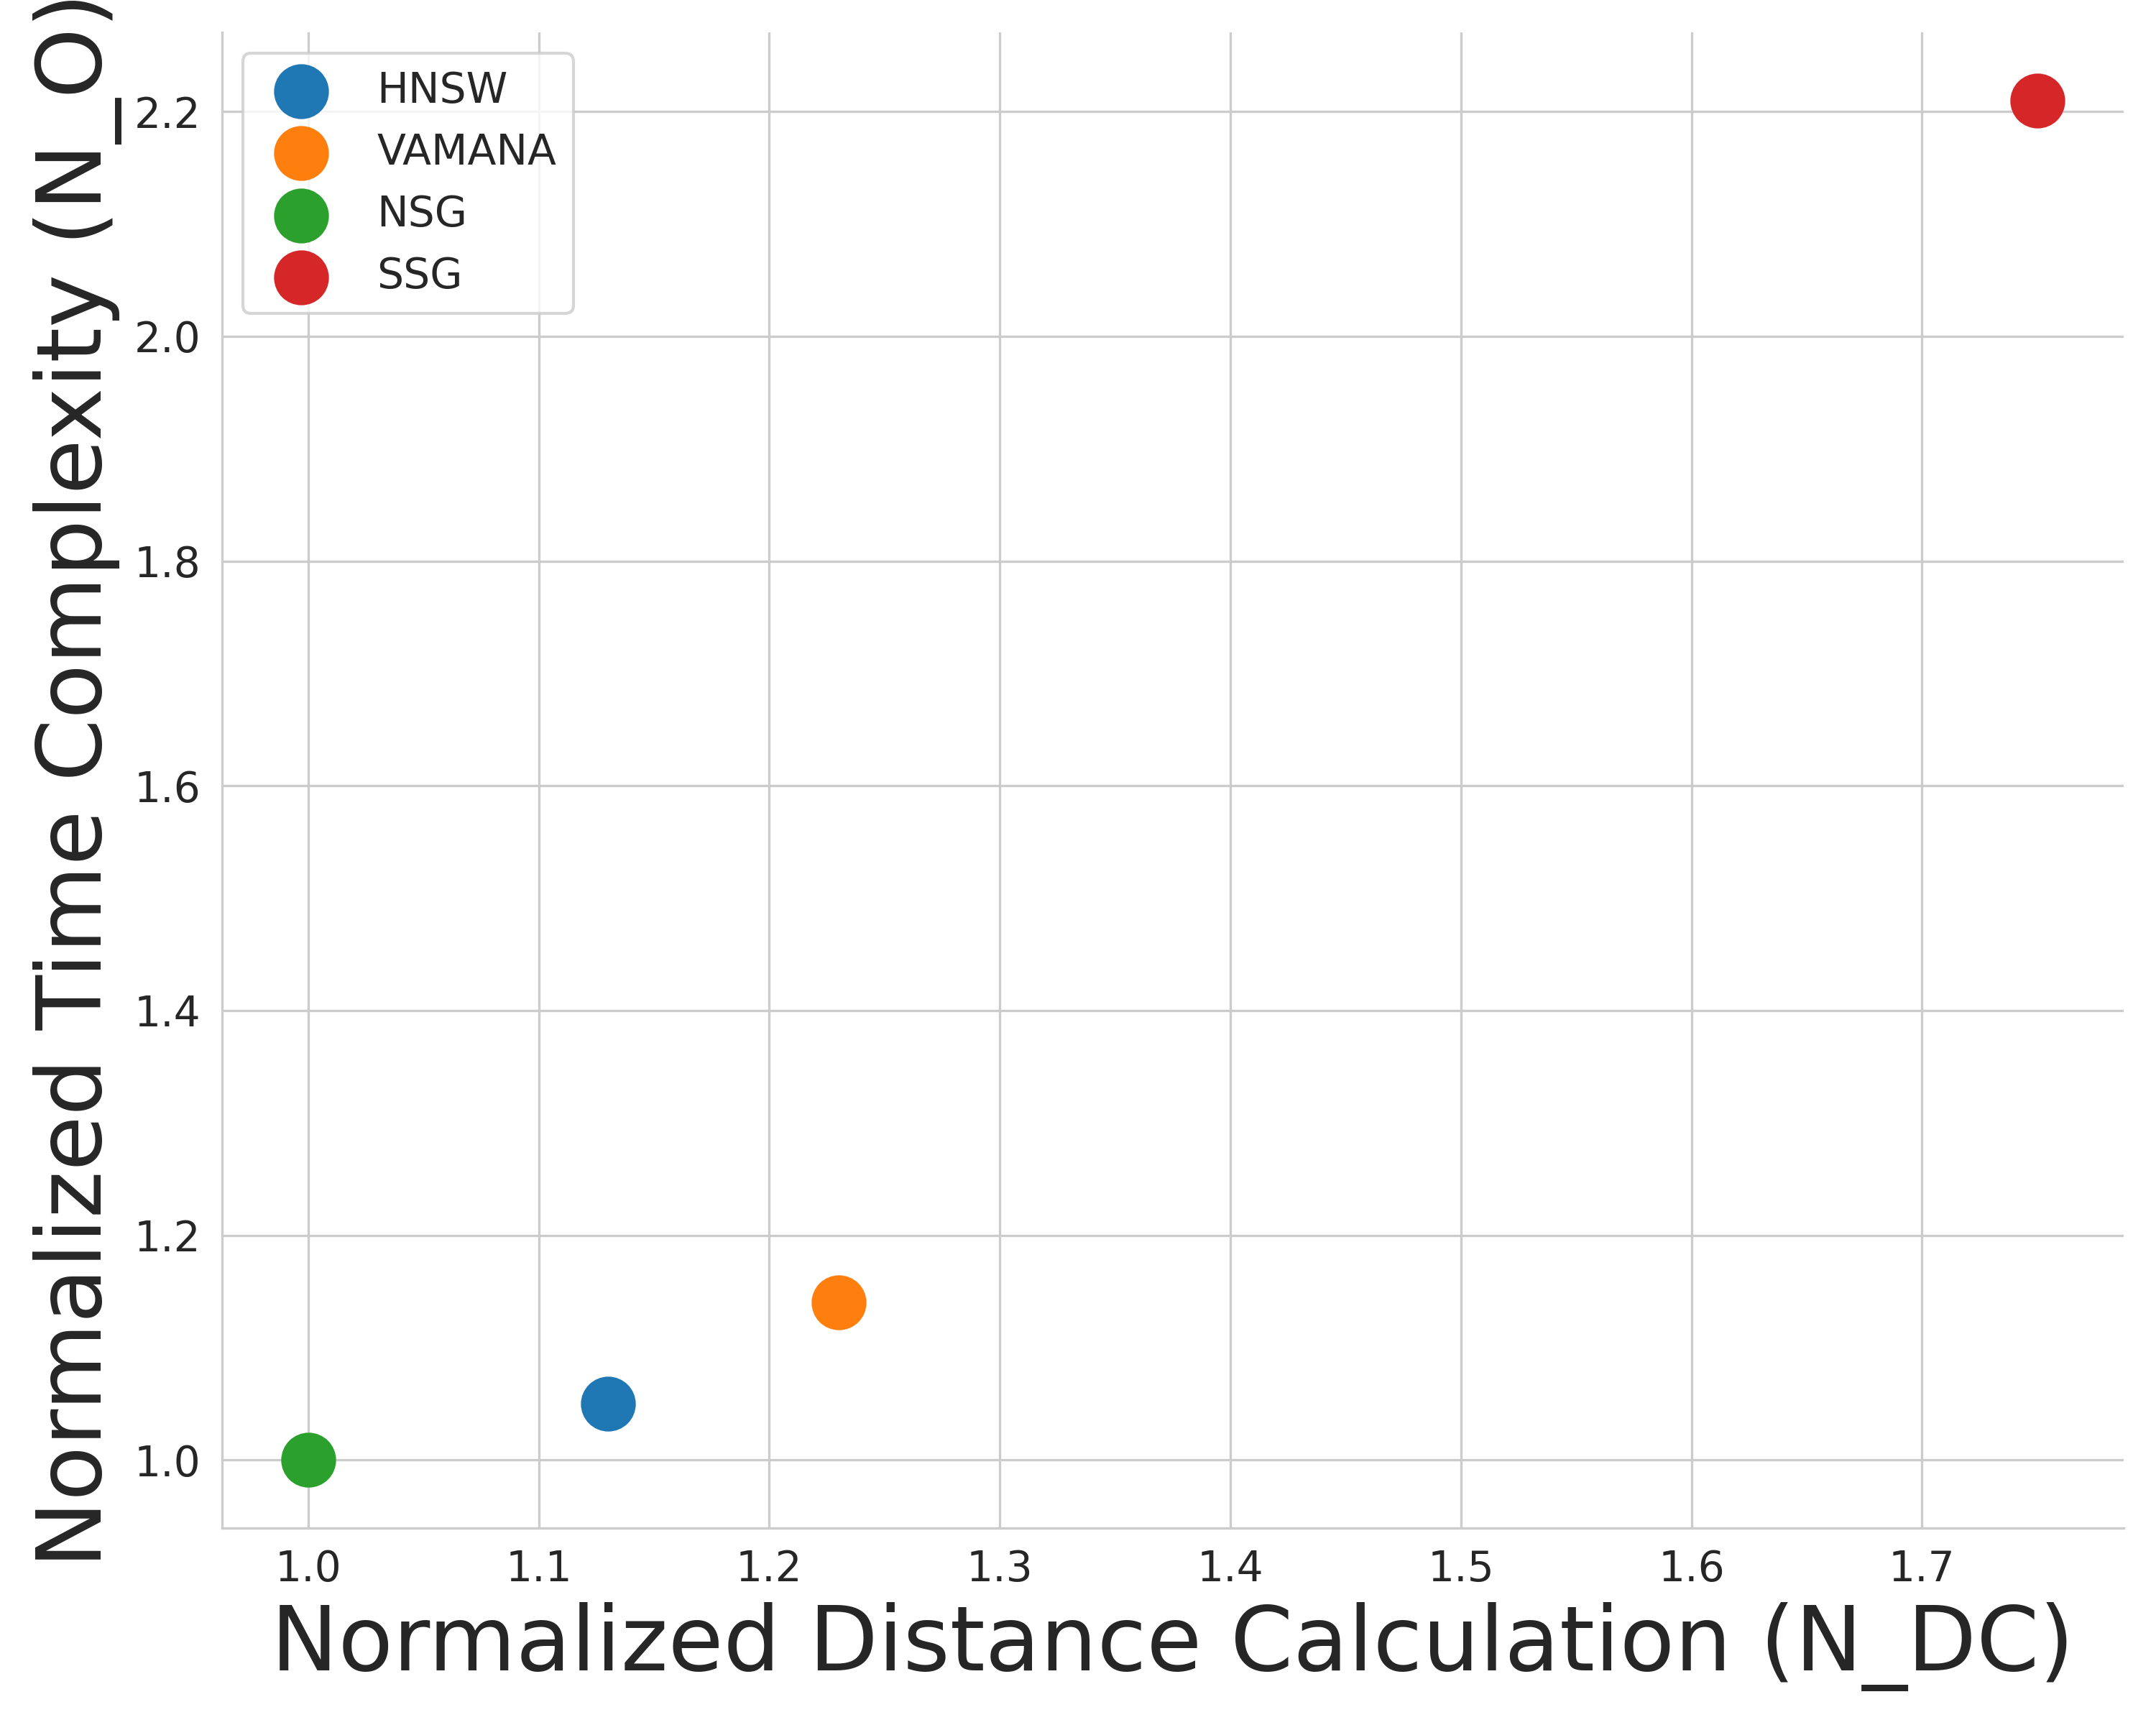
\includegraphics[width=\linewidth]{../img/Experiments/BSC/4_ndc_no.png}
  \caption{Deep4M}
  \label{fig:4_ndc_no}
\end{subfigure}
\hfill
\begin{subfigure}{0.24\textwidth}
  \centering
  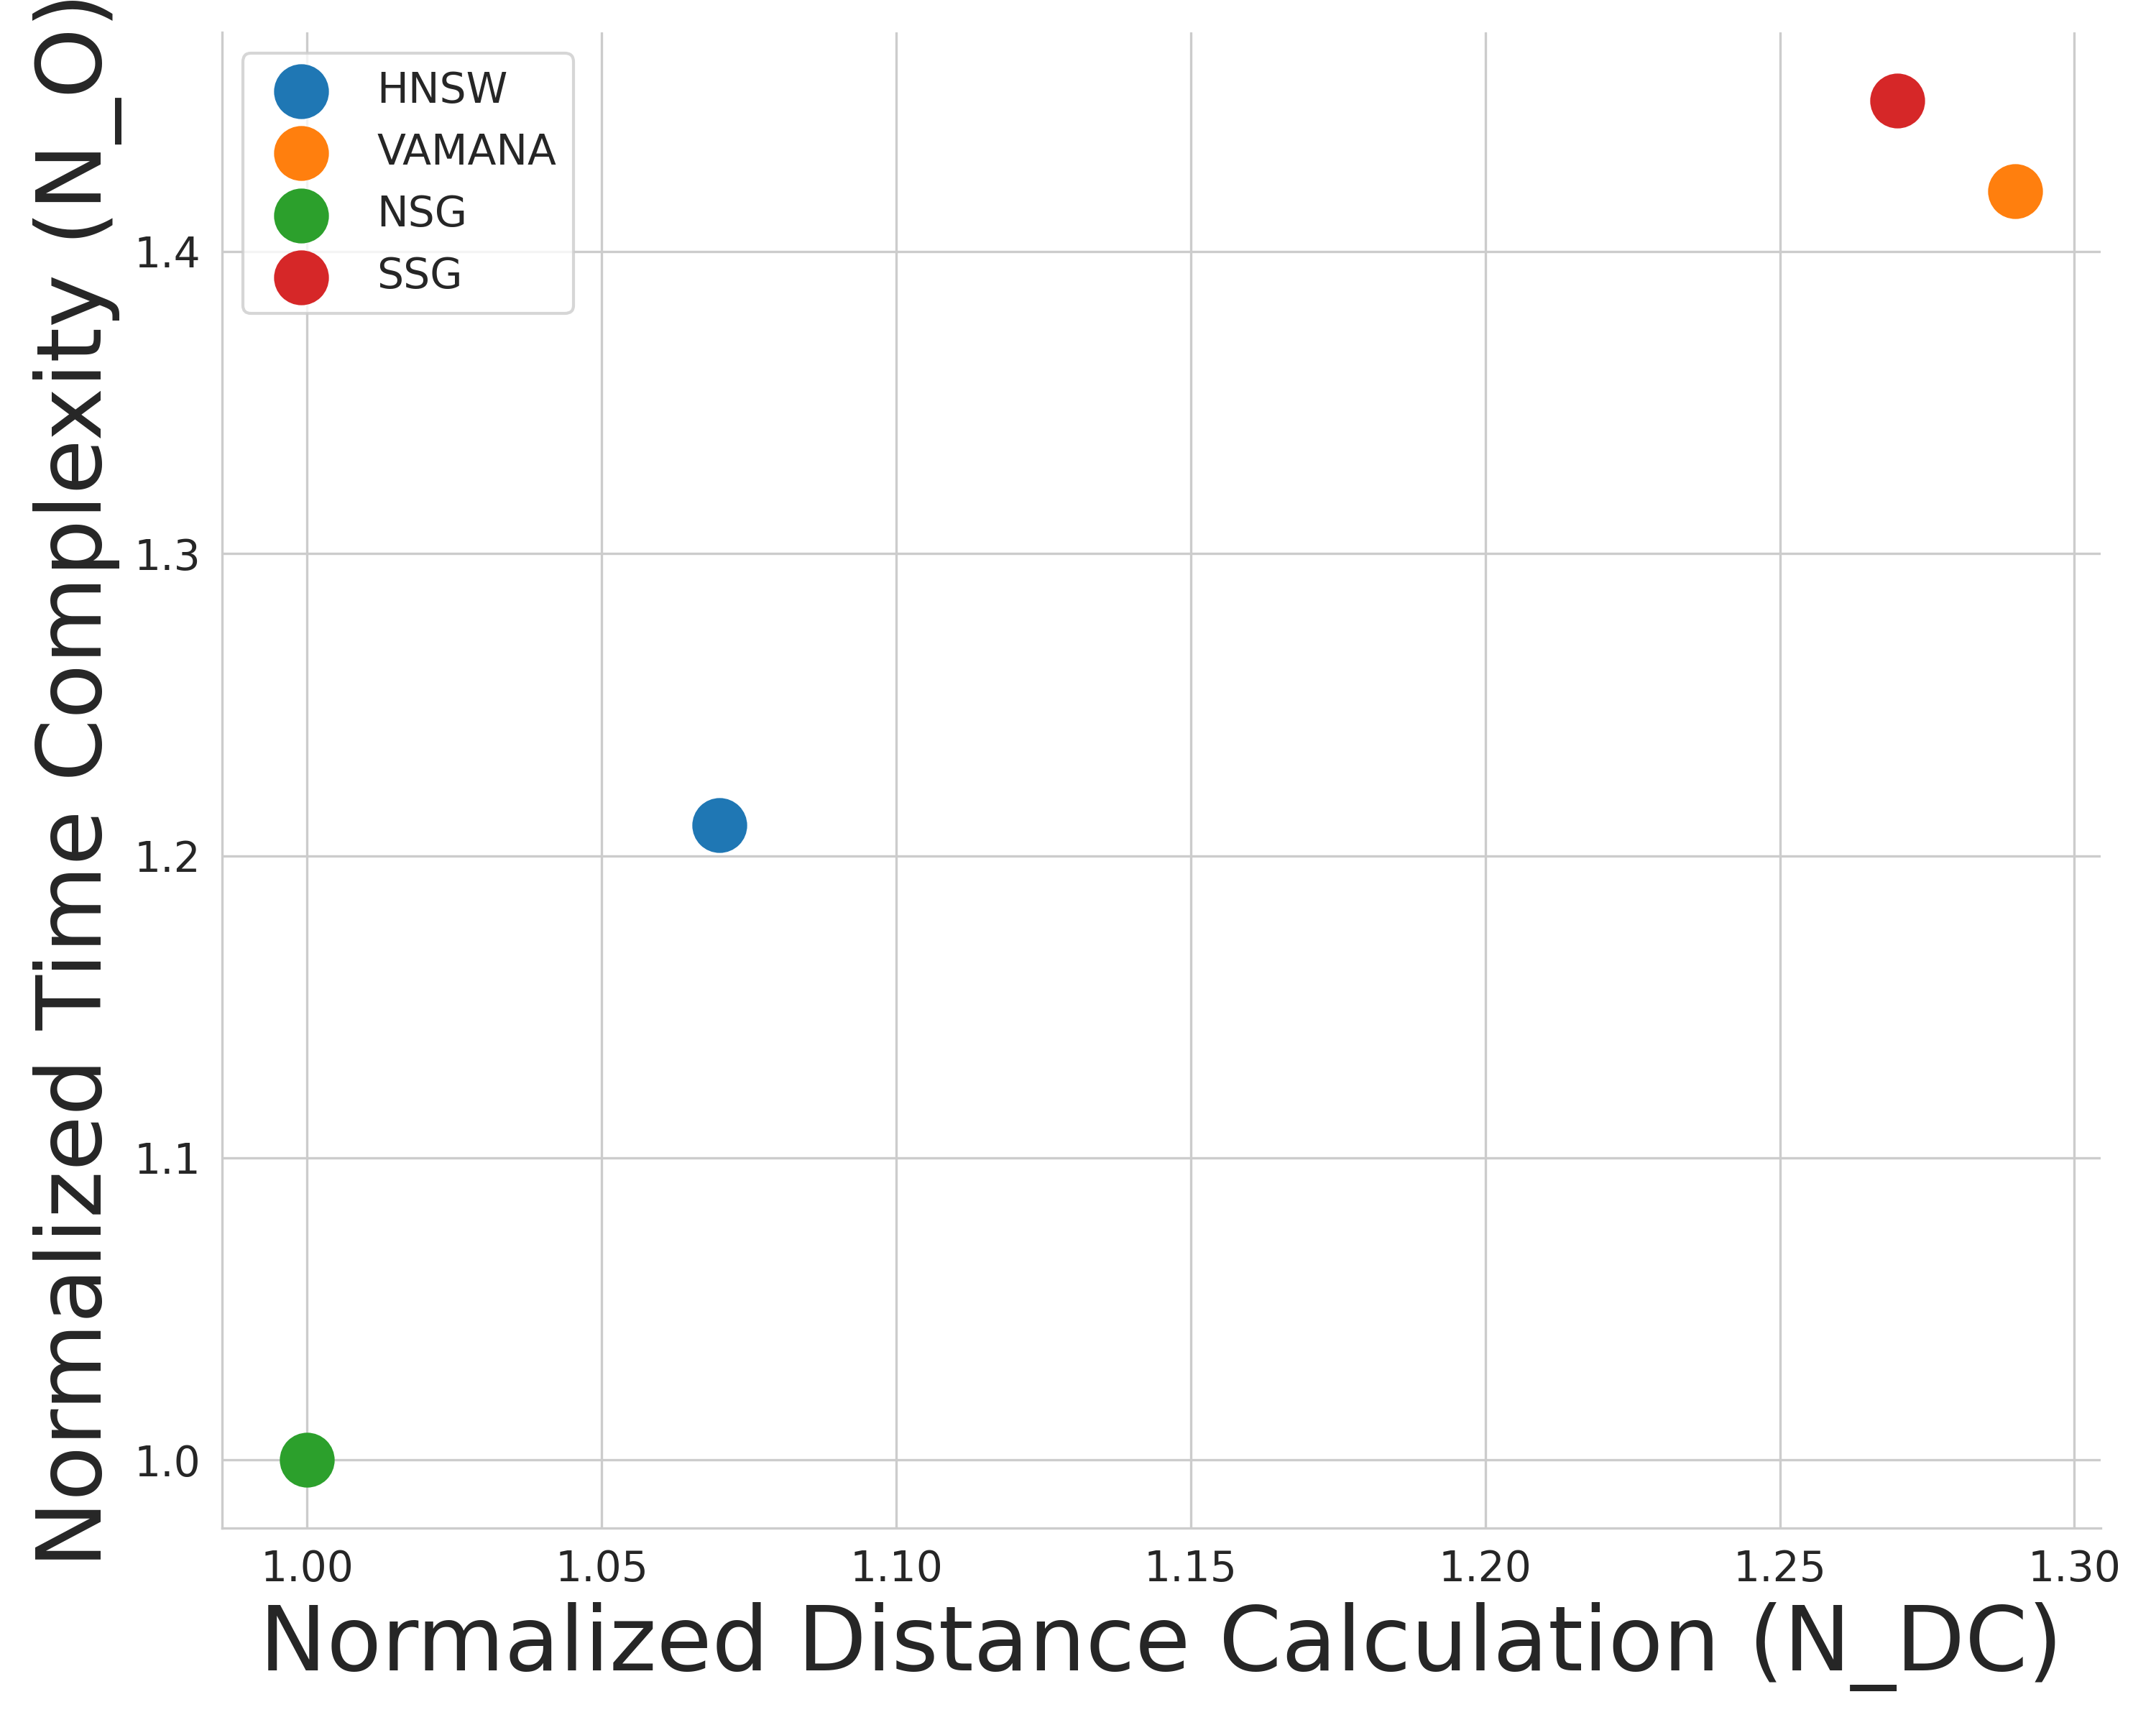
\includegraphics[width=\linewidth]{../img/Experiments/BSC/8_ndc_no.png}
  \caption{Deep8M}
  \label{fig:8_ndc_no}
\end{subfigure}
\caption{Normalized Distance Calculation (N\_DC) vs Normalized Time Complexity (N\_O) across different Deep1B dataset sizes}
\label{fig:ndc_no_plots}
\end{figure}



\end{comment}

\section{Conclusion}
In this chapter, we presented various state-of-the-art approaches for graph-based approximate vector search, along with a brief introduction to our proposed method, ELPIS. We also introduced a comprehensive taxonomy of graph-based methods, which we believe will aid the research community in understanding the key paradigms of current techniques while highlighting opportunities for further advancements in graph-based methods for vector search. 

Additionally, we provided an in-depth analysis of how Seed Selection strategies and Neighborhood Diversification (ND) methods affect graph search and indexing performance. We also explored how the theoretical complexity of the beam search algorithm translates into empirical performance during graph search. 

In the next chapter, we will delve deeper into the details of our ELPIS approach and compare its indexing and search performance with existing state-of-the-art graph methods on both real-world and synthetic datasets.

